\documentclass[aspectratio=169,9pt]{beamer}
\usepackage[utf8]{inputenc}
\usepackage{amsmath,amssymb,amsfonts,pgfpages,graphicx,subfigure,xcolor,bm,multirow,microtype,wasysym,multimedia,hyperref,tabularx,amscd,pgfgantt,mhchem,physics}

\usetikzlibrary{shapes.gates.logic.US,trees,positioning,arrows,shapes.geometric}
\usepackage{mathpazo,libertine}
\usepackage{smartdiagram}
\usepackage{comment}

\definecolor{darkgreen}{RGB}{0, 180, 0}

% coordinates
\newcommand{\br}{\mathbf{r}}

% methods
\newcommand{\evGW}{ev$GW$}
\newcommand{\qsGW}{qs$GW$}
\newcommand{\GOWO}{$G_0W_0$}
\newcommand{\Hxc}{\text{Hxc}}
\newcommand{\xc}{\text{xc}}
\newcommand{\Ha}{\text{H}}
\newcommand{\co}{\text{x}}

\newcommand{\violet}[1]{\textcolor{lavender}{#1}}
\newcommand{\orange}[1]{\textcolor{orange}{#1}}
\newcommand{\purple}[1]{\textcolor{purple}{#1}}
\newcommand{\blue}[1]{\textcolor{blue}{#1}}
\newcommand{\green}[1]{\textcolor{darkgreen}{#1}}
\newcommand{\yellow}[1]{\textcolor{fooyellow}{#1}}
\newcommand{\red}[1]{\textcolor{red}{#1}}
\newcommand{\highlight}[1]{\textcolor{fooblue}{#1}}

\newcommand{\pub}[1]{{\small \textcolor{purple}{#1}}}


\institute{Laboratoire de Chimie et Physique Quantiques, IRSAMC, UPS/CNRS, Toulouse \\
\url{https://lcpq.github.io/pterosor}}
\usetheme{pterosor}
\author{F\'abris Kossoski}  
\date{24/05/2022} 
\title{New methods for excited states}  

\begin{document}

\maketitle


%%%%%%%%%%%%%%%%%%%%%%%%%%%%%%%%%%%%%%%%%%%%
\begin{frame}{General overview of the PTEROSOR team}
        \centering
        \begin{columns}
                \begin{column}{0.325\textwidth}
                        \centering
                        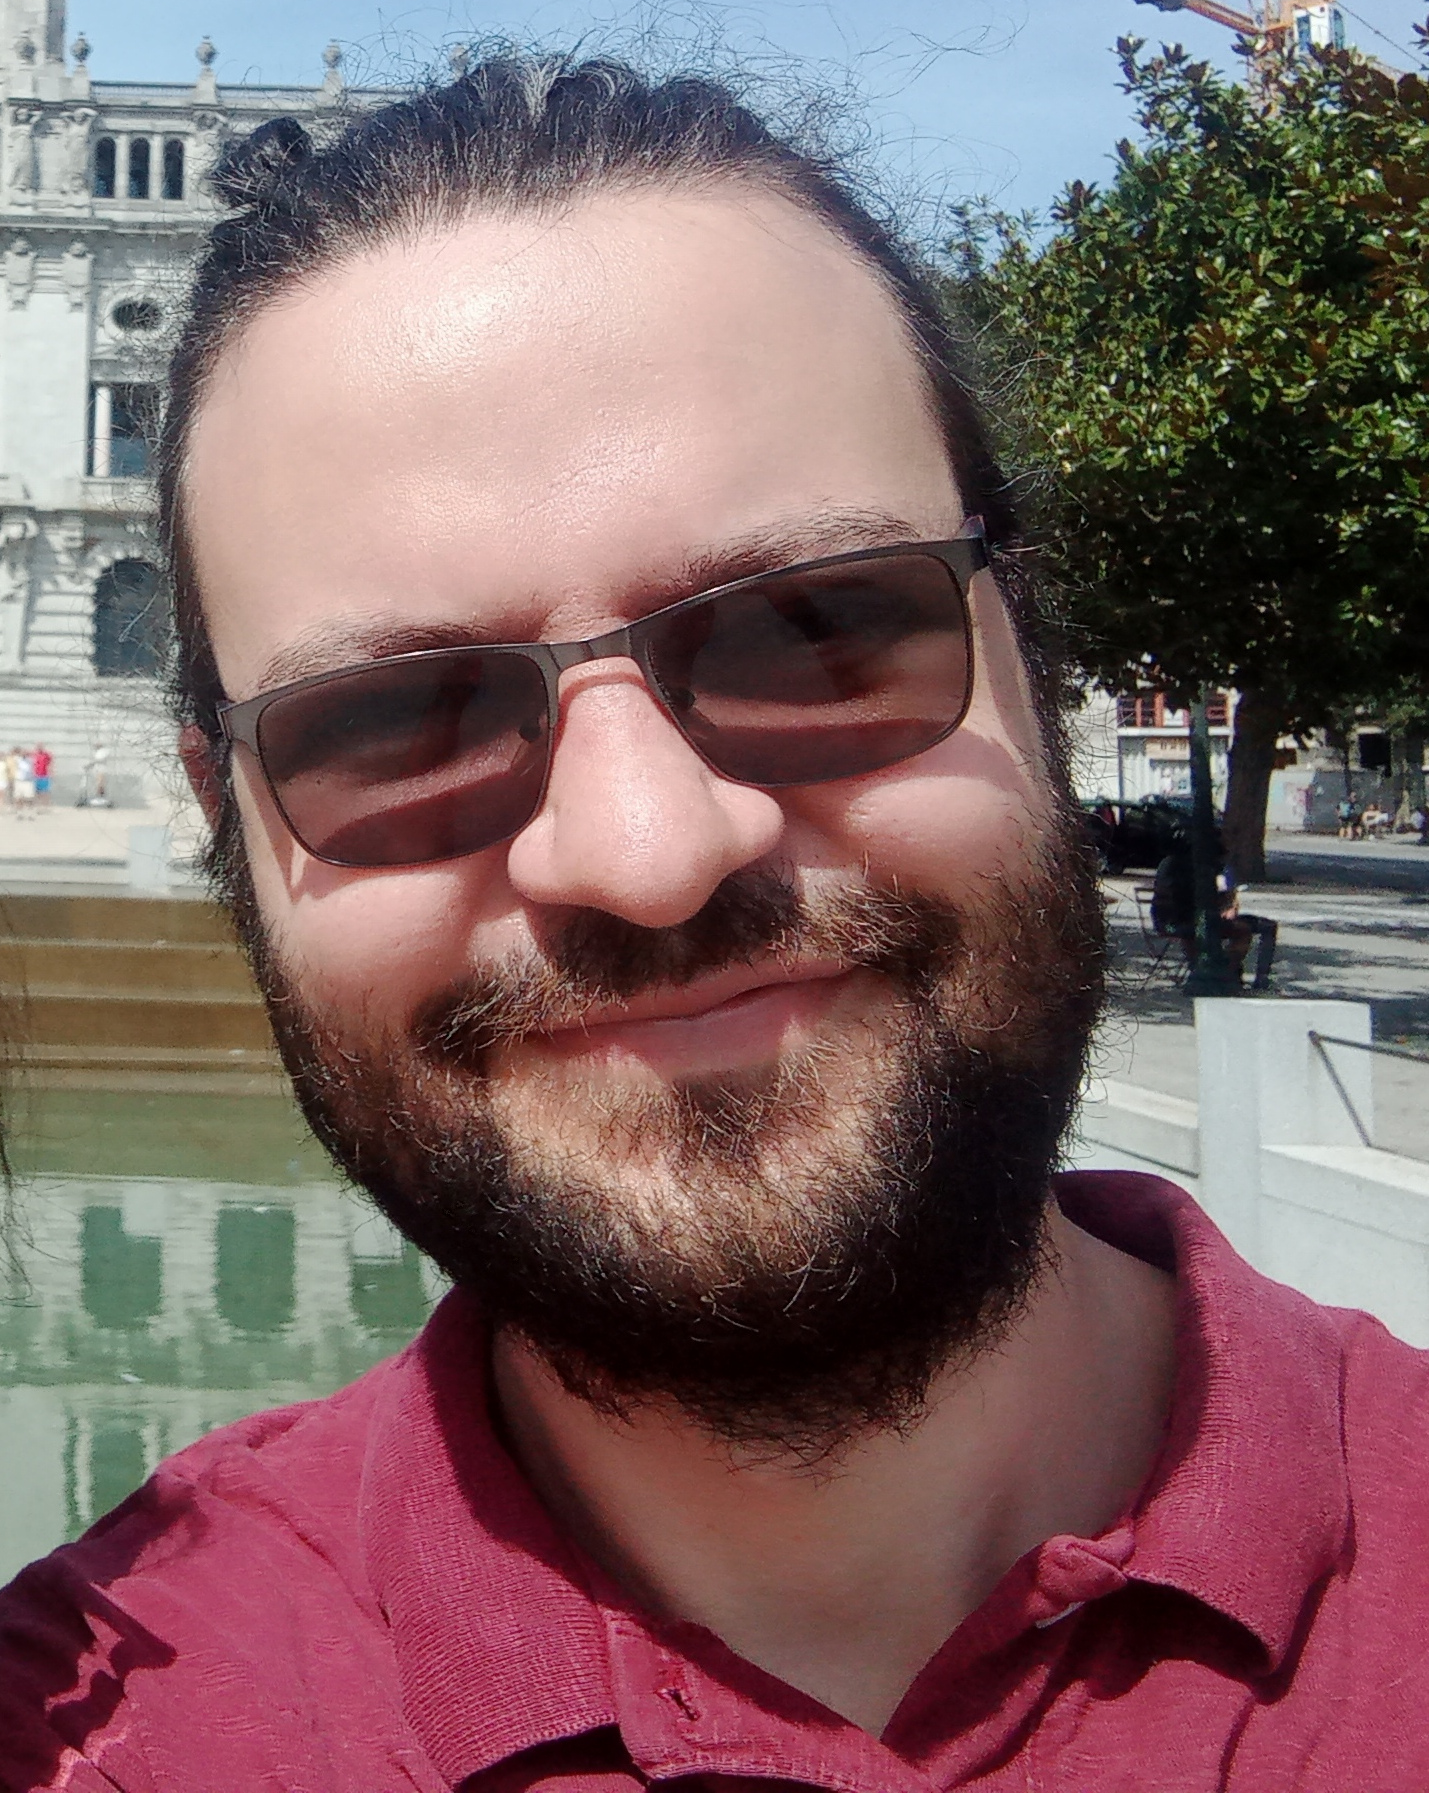
\includegraphics[width=0.3\textwidth]{fig/Fabris_2021.png}
                        \\
                        F\'abris Kossoski
                        \\
			\vspace{0.25cm}
                        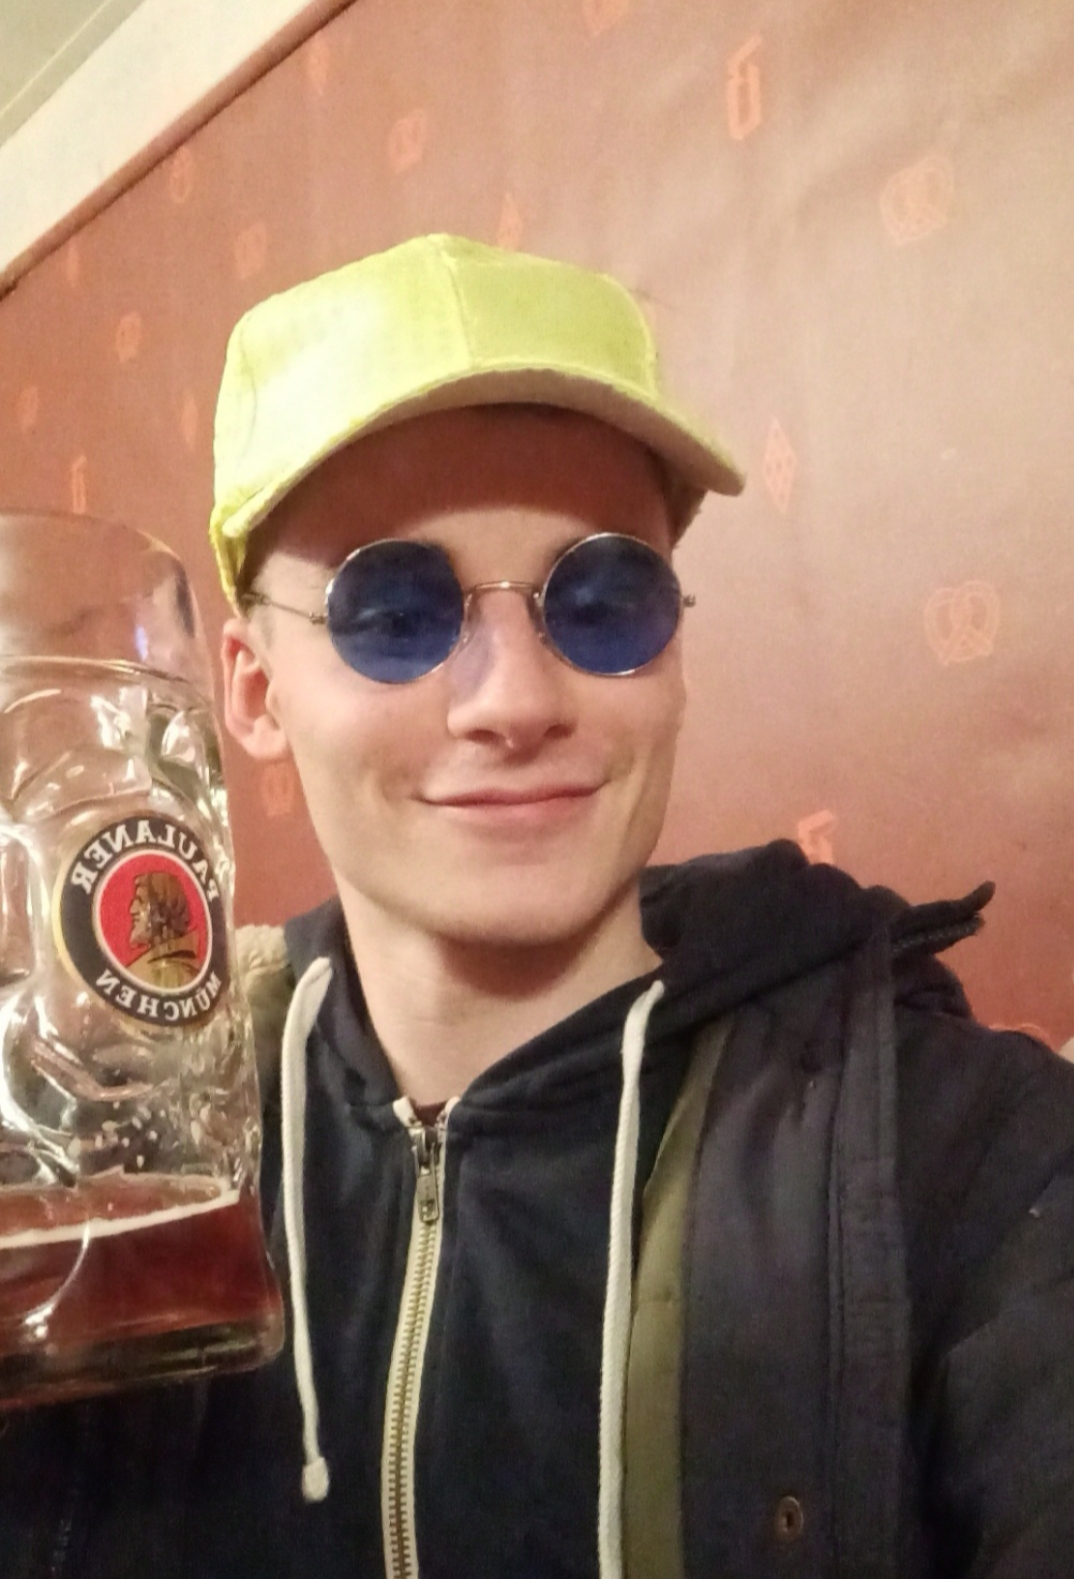
\includegraphics[width=0.3\textwidth]{fig/Yann.jpg}
                        \\
                        Yann Damour
                        \\
			\vspace{0.25cm}
                        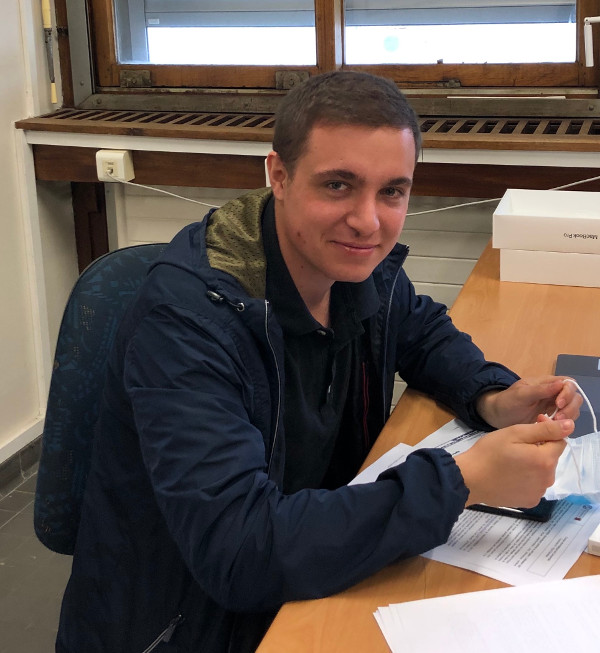
\includegraphics[width=0.3\textwidth]{fig/Enzo}
                        \\
                        Enzo Monino 
                        \\
                \end{column}
                \begin{column}{0.50\textwidth}
			\vspace{-0.5cm}
                 \smartdiagramset{distance planet-satellite=4cm}
                        \resizebox{\textwidth}{!}{
                                \smartdiagram[constellation diagram]{
                                        {\small Excited-State Methods (Anthony, Michel \& Titou)},
                                        {\small Selected CI (Yann \& Fabris) },
                                        {\small CC for Excited States (Antoine, Raul \& Fabris)},
                                        {\small ``Complex'' Quantum Chemistry (Antoine)},
                                        {\small Many-Body Perturbation Theory (Enzo \& Roberto)},
                                        {\small Ensemble DFT (Clotilde)},
                                        {\small QUEST database (Mika, Martial \& co)}
                                }
                        }
                \end{column}
                \begin{column}{0.325\textwidth}
                        \centering
                        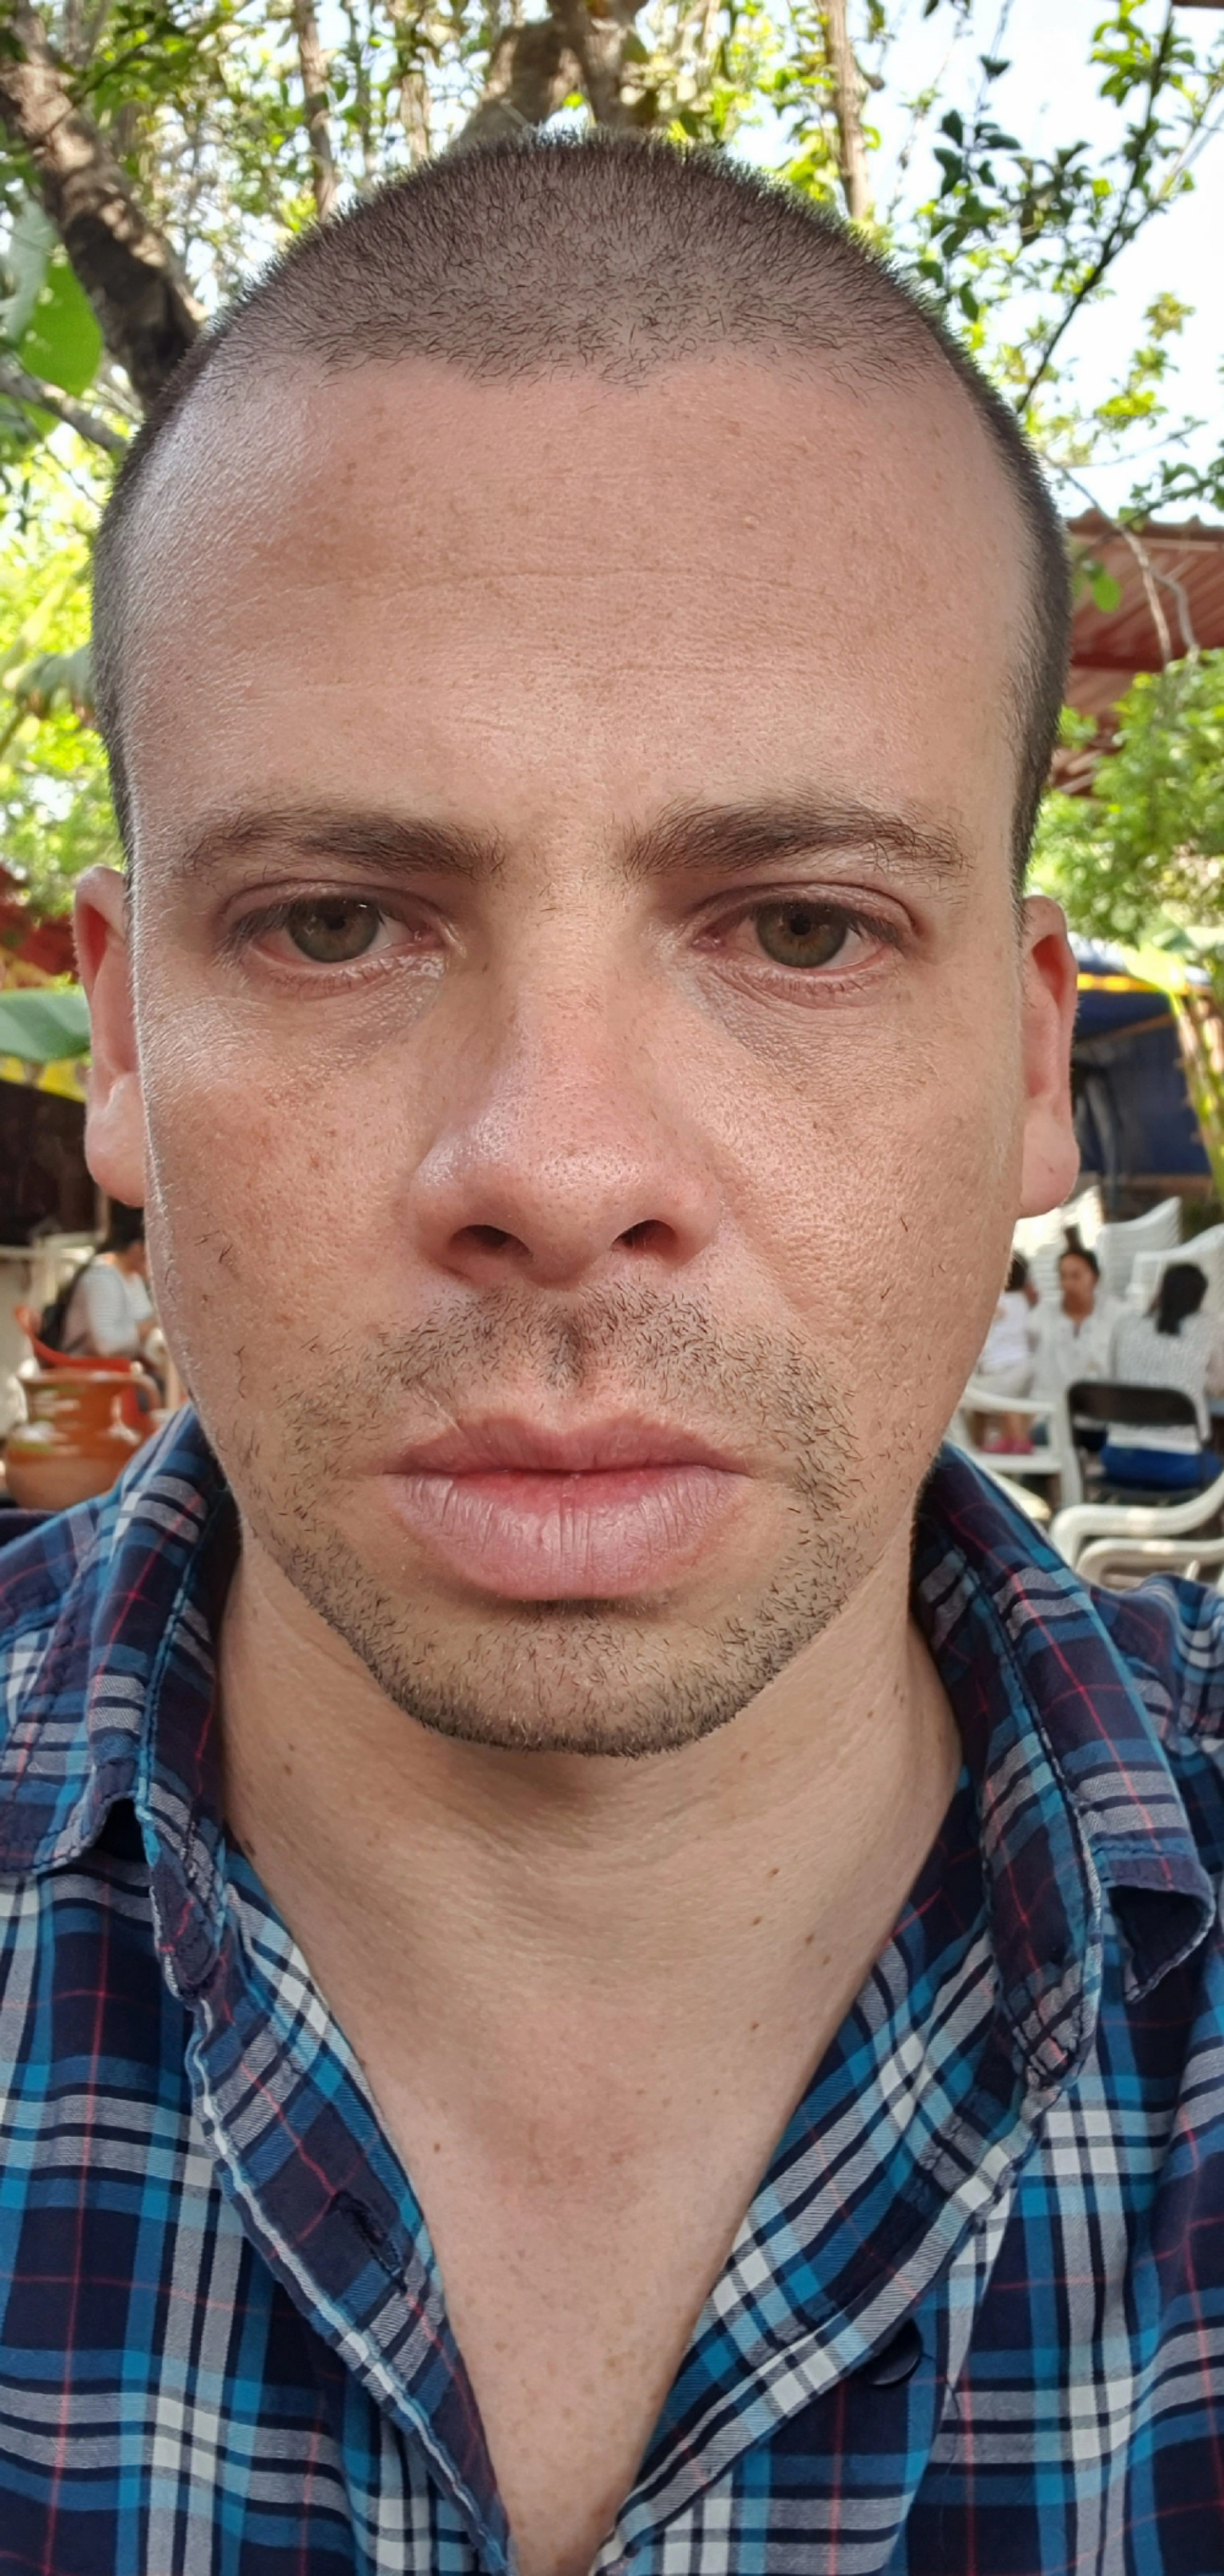
\includegraphics[width=0.2\textwidth]{fig/Raul}
                        \\
                        Raul Quintero
                        \\
			\vspace{0.25cm}
                        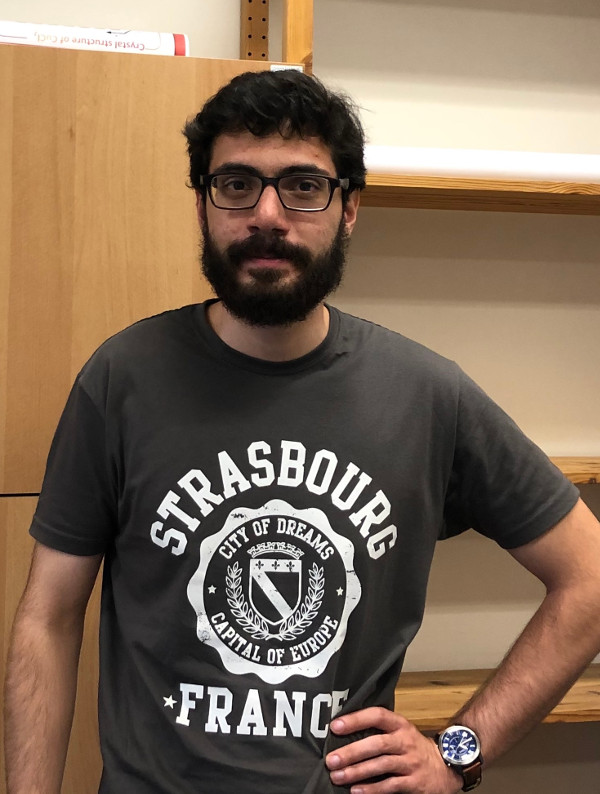
\includegraphics[width=0.3\textwidth]{fig/Roberto}
                        \\
                        Roberto Orlando
                        \\
			\vspace{0.25cm}
                        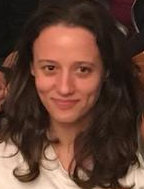
\includegraphics[width=0.3\textwidth]{fig/Clotilde}
                        \\
                        Clotilde Marut
                        \\
                \end{column}
        \end{columns}
			\vspace{-0.5cm}
        \url{https://lcpq.github.io/PTEROSOR/}
\end{frame}
%%%%%%%%%%%%%%%%%%%%%%%%%%%%%%%%%%%%%%%%%%%%


%%%%%%%%%%%%%%%%%%%%%%%%%%%%%%%%%%%%%%%%%%%%
\begin{frame}{Highly-accurate excitation energies: The QUEST project}
    \begin{center}
        \textit{\green{``The aim of the QUEST project is to provide to the community a large set of highly-accurate excitation energies for various types of excited states''}}
    \end{center}
			\vspace{-0.35cm}
        \begin{columns}
                \begin{column}{0.40\textwidth}
                        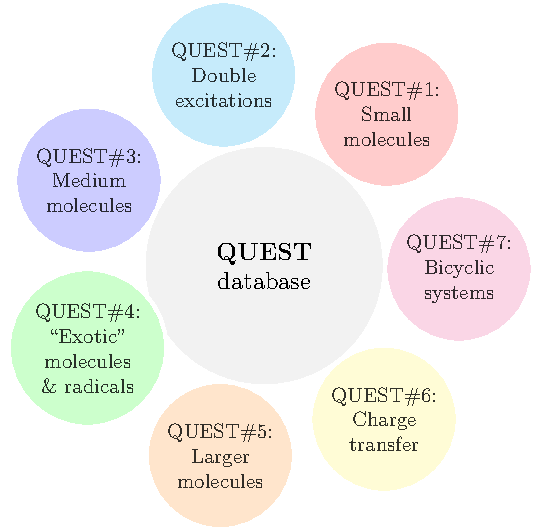
\includegraphics[width=1.10\textwidth]{fig/QUEST.pdf}
                \end{column}
                \begin{column}{0.40\textwidth}
                        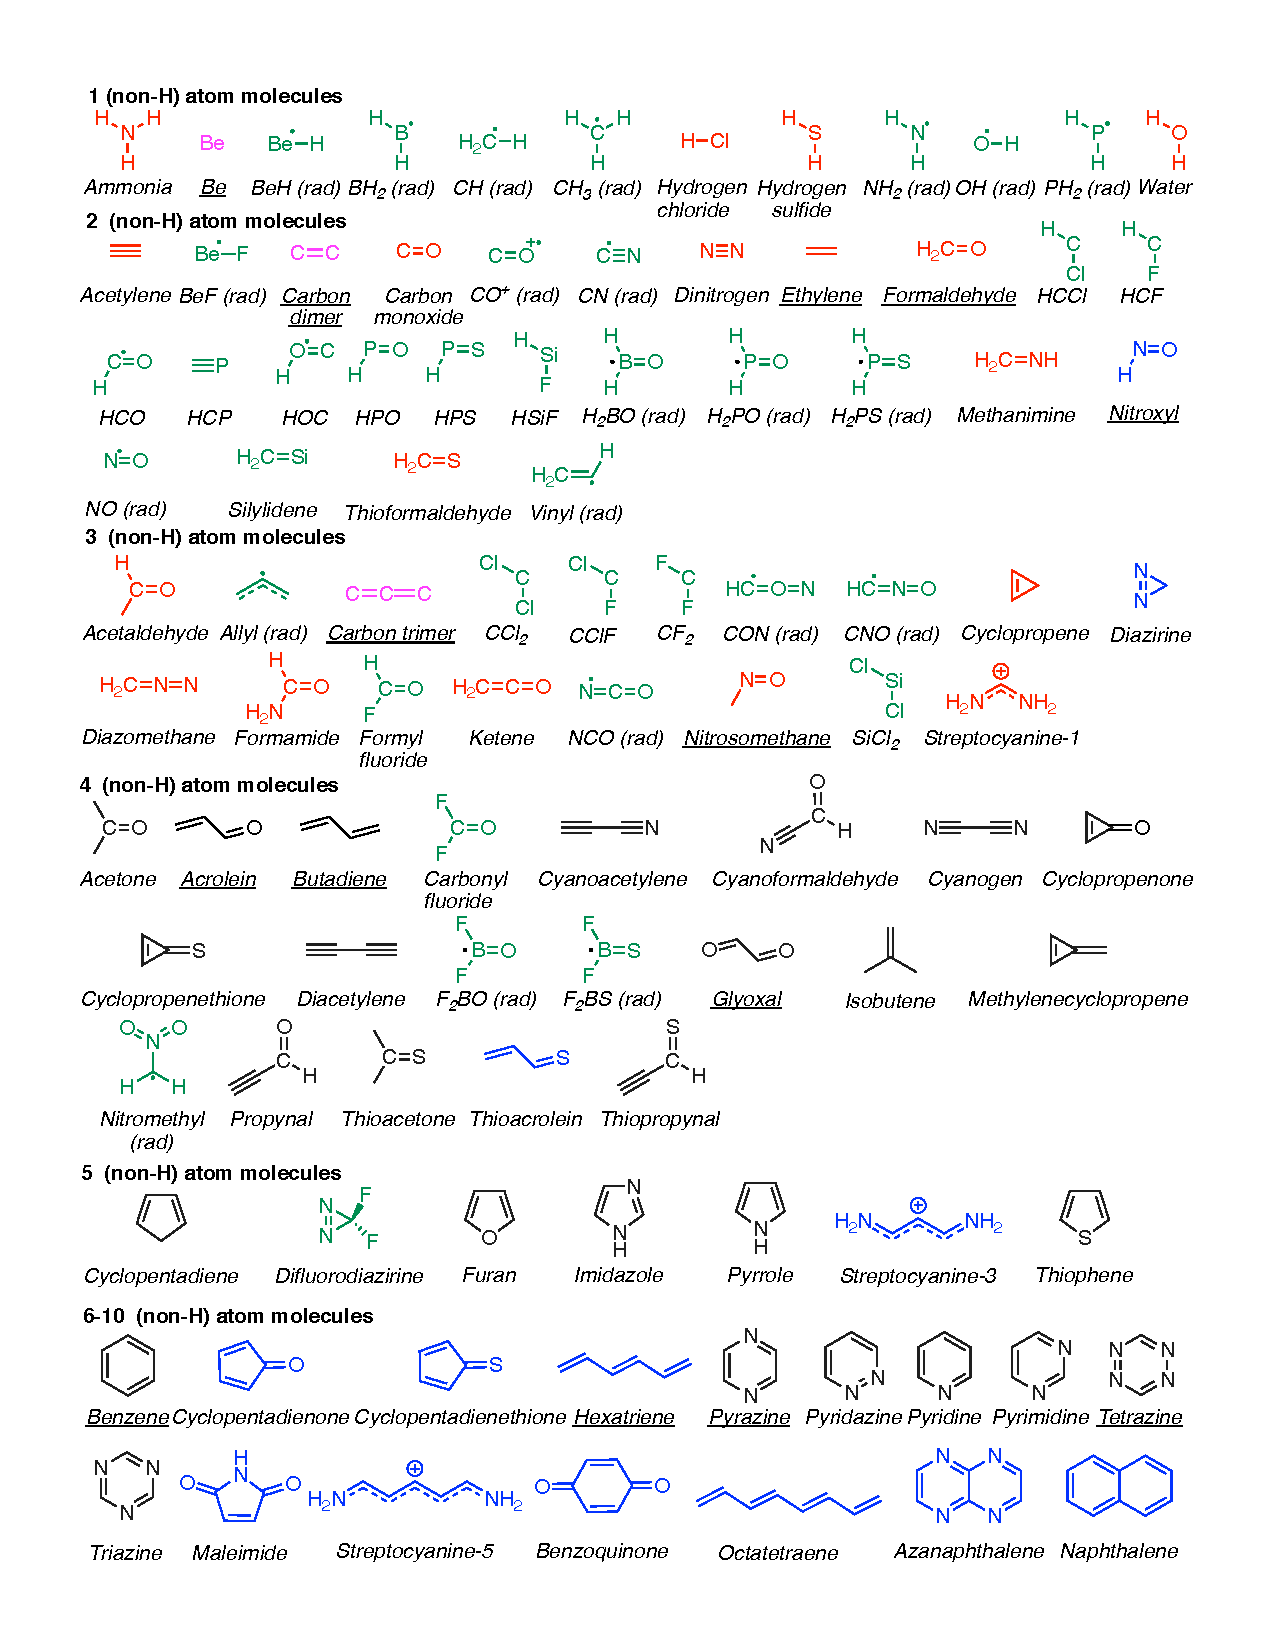
\includegraphics[width=0.95\textwidth]{fig/QUEST_mol}
                \end{column}
                \begin{column}{0.20\textwidth}
                        \centering
                        \small
                        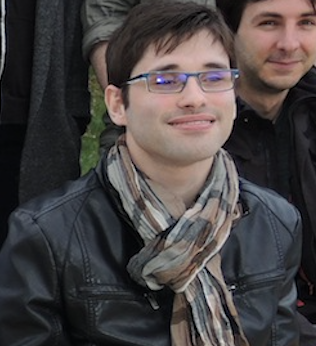
\includegraphics[width=0.6\textwidth]{fig/Mika}
                        \\
                        Mika Veril
                         \\
                         \bigskip
                        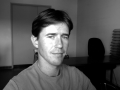
\includegraphics[width=0.6\textwidth]{fig/Martial}
                        \\
                        Martial Boggio-Pasqua
                         \\
                         \bigskip
                        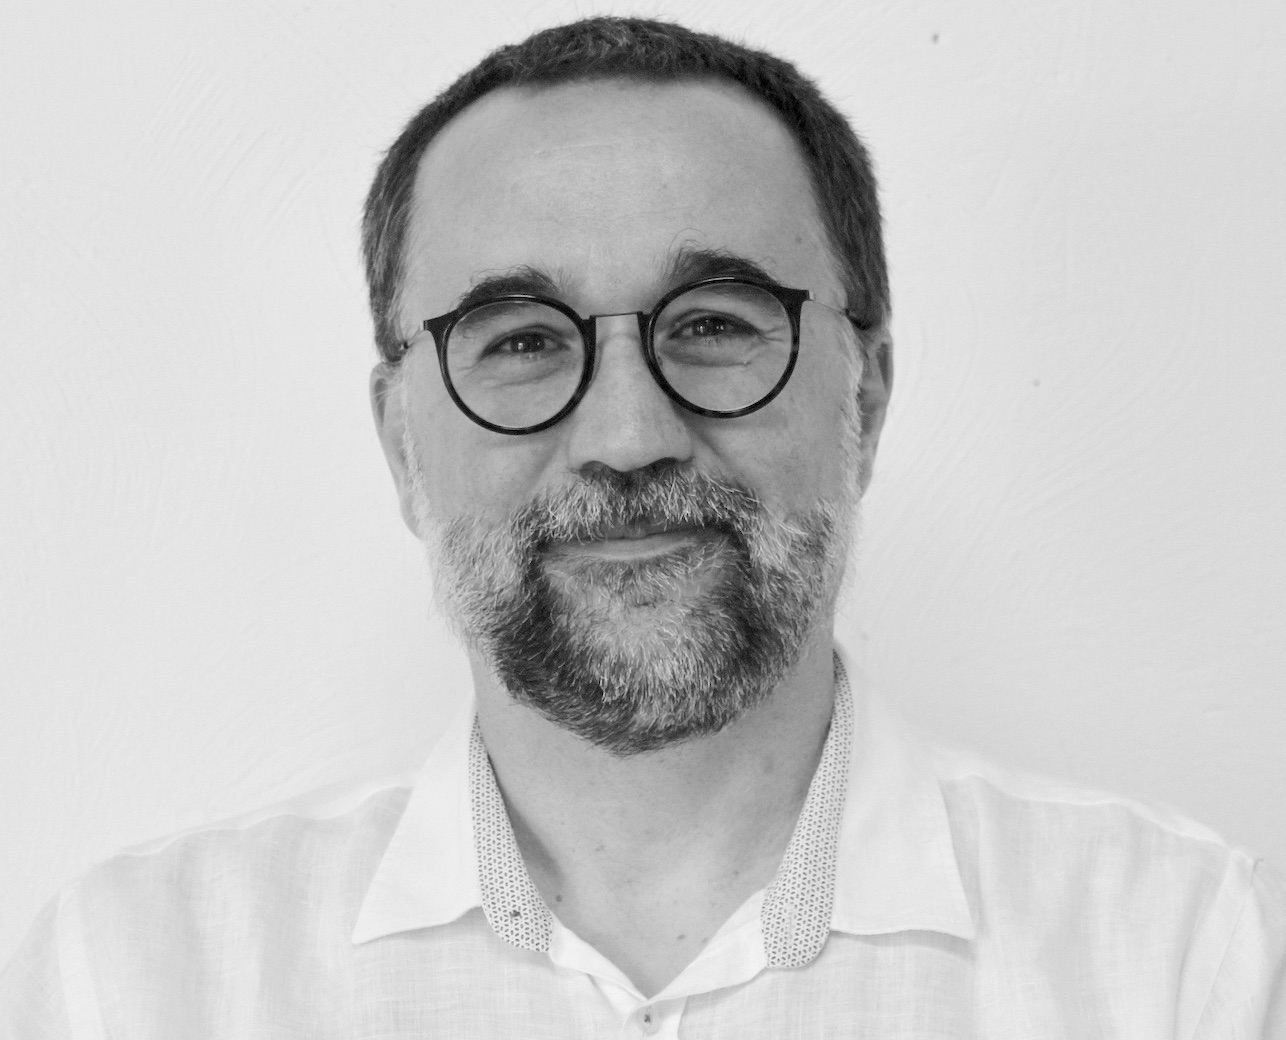
\includegraphics[width=0.6\textwidth]{fig/Denis}
                        \\
                        Denis Jacquemin
                \end{column}
        \end{columns}
\end{frame}
%%%%%%%%%%%%%%%%%%%%%%%%%%%%%%%%%%%%%%%%%%%%


%%%%%%%%%%%%%%%%%%%%%%%%%%%%%%%%%%%%%%%%%%%%
\begin{frame}{Highly-accurate excitation energies: The QUEST project}
        \begin{center}
                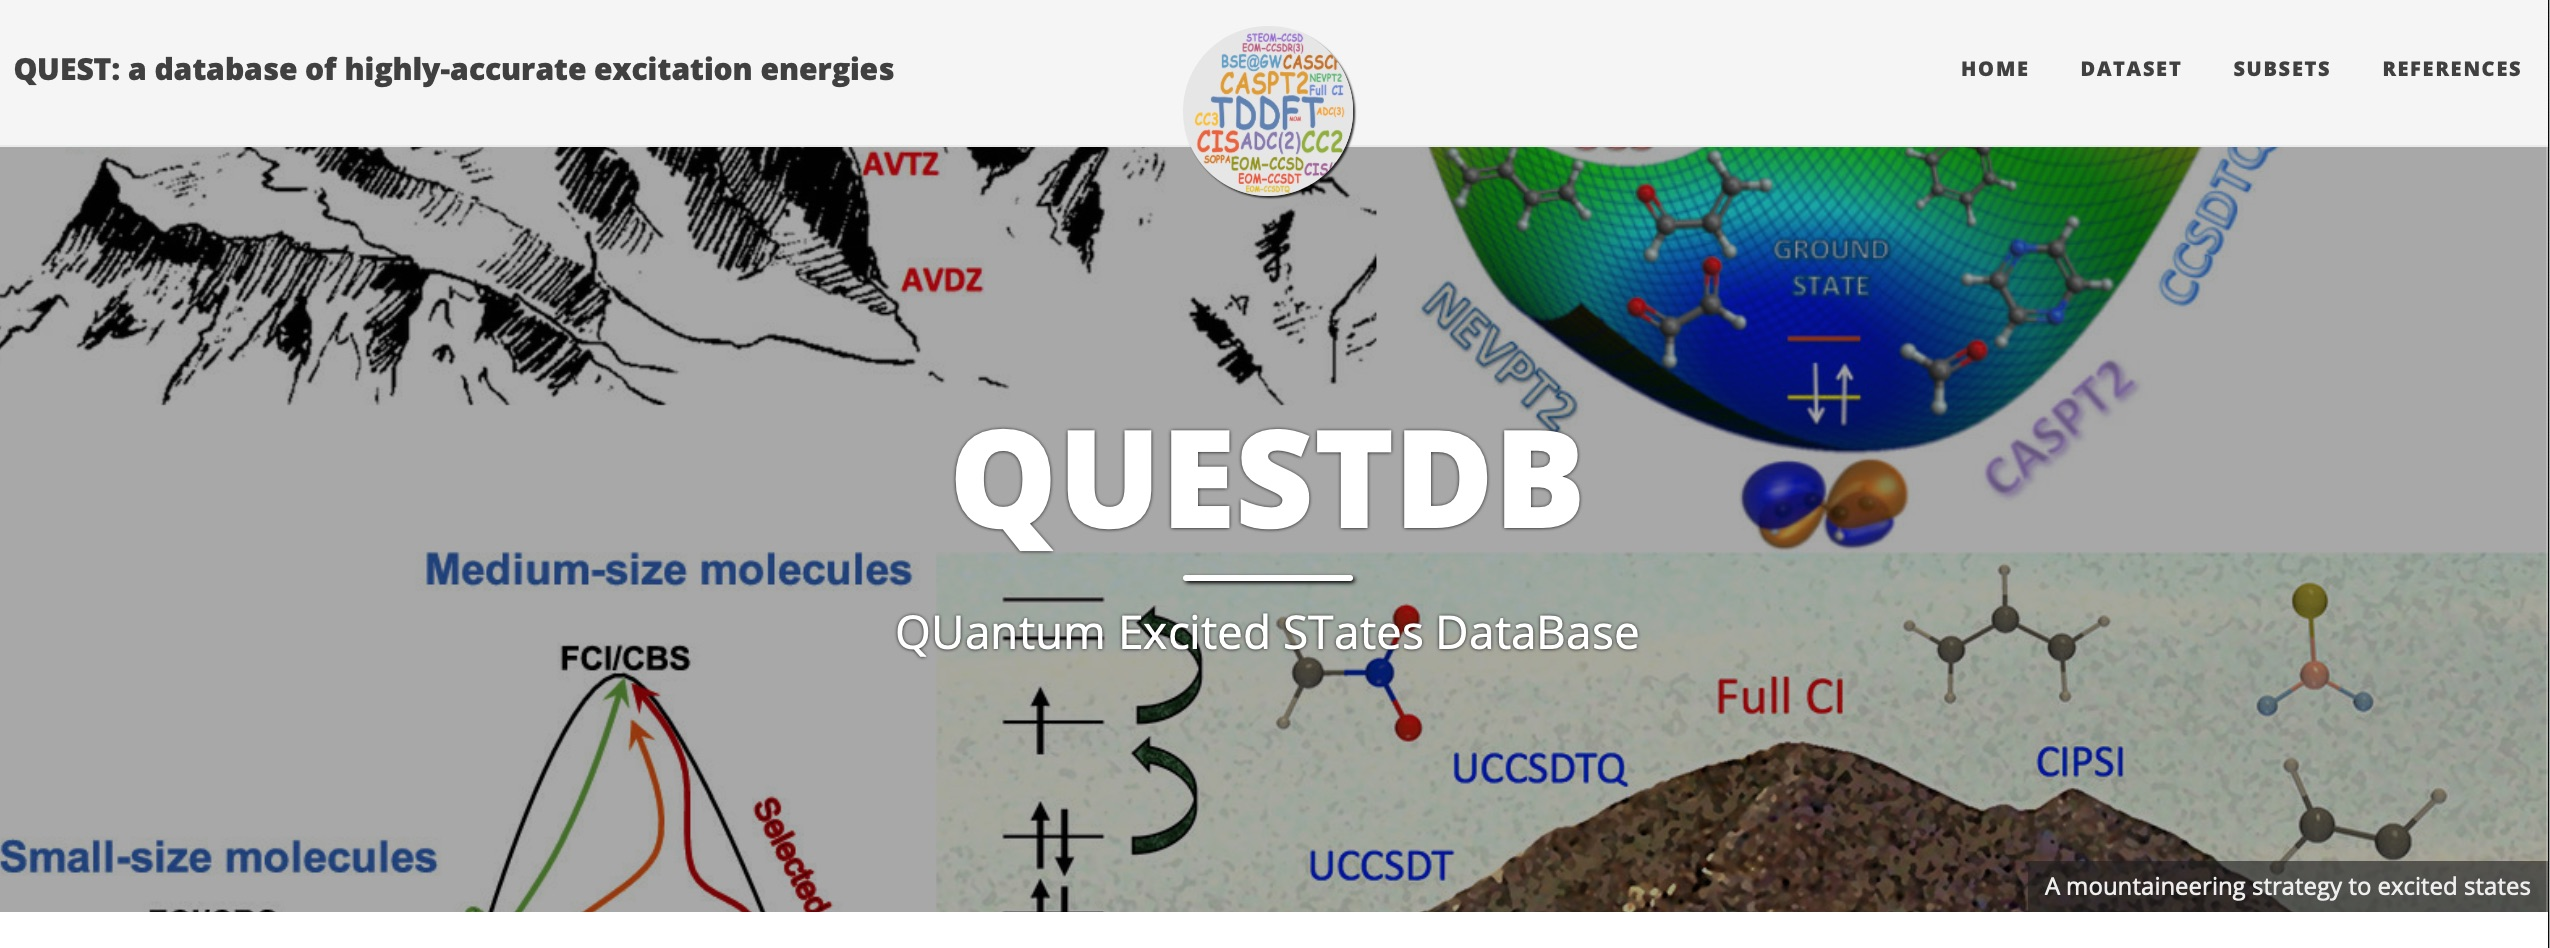
\includegraphics[width=0.9\textwidth]{fig/TOC_QUEST}
                \\
                \bigskip
                \url{https://lcpq.github.io/QUESTDB_website/}
                \\
                \bigskip
		\pub{WIREs Comput. Mol. Sci. e1517 (2021)}
        \end{center}
\end{frame}
%%%%%%%%%%%%%%%%%%%%%%%%%%%%%%%%%%%%%%%%%%%%


%%%%%%%%%%%%%%%%%%%%%%%%%%%%%%%%%%%%%%%%%%%%
\begin{frame}{Quantum Package 2.0}
        \begin{columns}
                \begin{column}{0.80\textwidth}
                    \centering
                    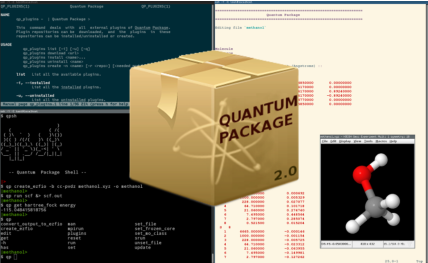
\includegraphics[width=0.75\textwidth]{fig/TOC_QP2}
                \end{column}
                \begin{column}{0.20\textwidth}
                        %\centering
                        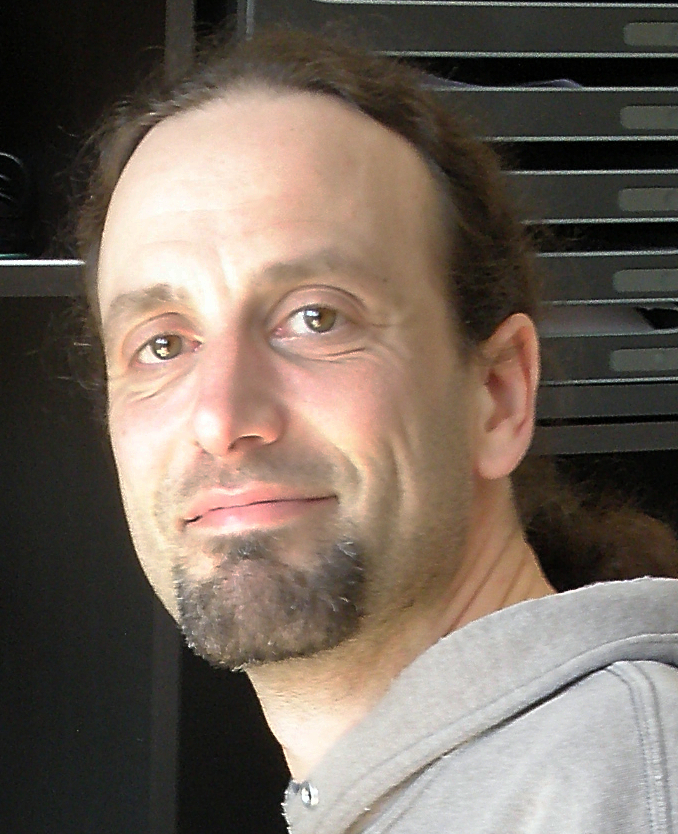
\includegraphics[width=0.8\textwidth]{fig/Anthony}
                        \\
                        Anthony Scemama
                \end{column}
        \end{columns}
        \centering
        \bigskip
    	\url{https://github.com/QuantumPackage/qp2}
        \\
        \bigskip
        {\em ``Quantum Package 2.0: An Open-Source Determinant-Driven Suite of Programs''}\\
        \bigskip
	\pub{JCTC 15, 3591 (2019)}
\end{frame}
%%%%%%%%%%%%%%%%%%%%%%%%%%%%%%%%%%%%%%%%%%%%


%%%%%%%%%%%%%%%%%%%%%%%%%%%%%%%%%%%%%%%%%%%%
\begin{frame}{Orbital optimized selected CI}

\begin{columns}

\begin{column}{0.5\textwidth}

\centering
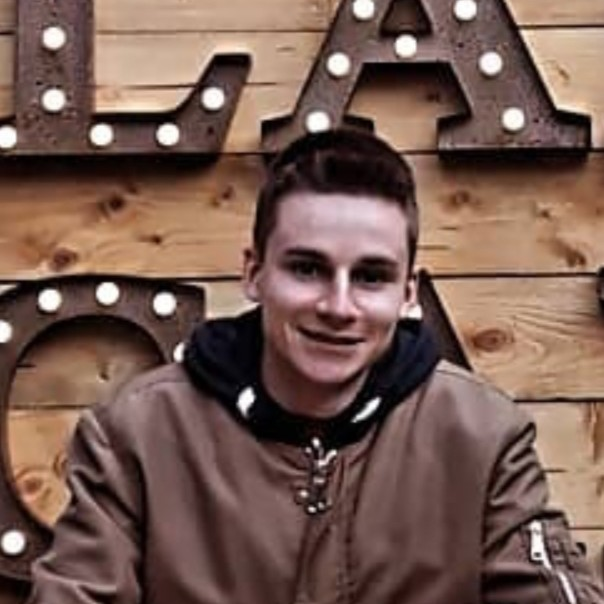
\includegraphics[width=0.4\textwidth]{fig/Yann2.jpg}
\\
Yann Damour
\\

\begin{itemize}
	\item Orbital optimization largely accelerates the convergence of selected CI
                        \bigskip
	\item Trust-region Newton-Raphson algorithm
                        \bigskip
\end{itemize}
			\bigskip
                        \centering
			\pub{JCP 155, 134104 (2021)}
\end{column}

                \begin{column}{0.5\textwidth}
                        \centering
			\begin{block}{Variational energy for different sets of orbitals (Benzene / cc-pVDZ)}
                        %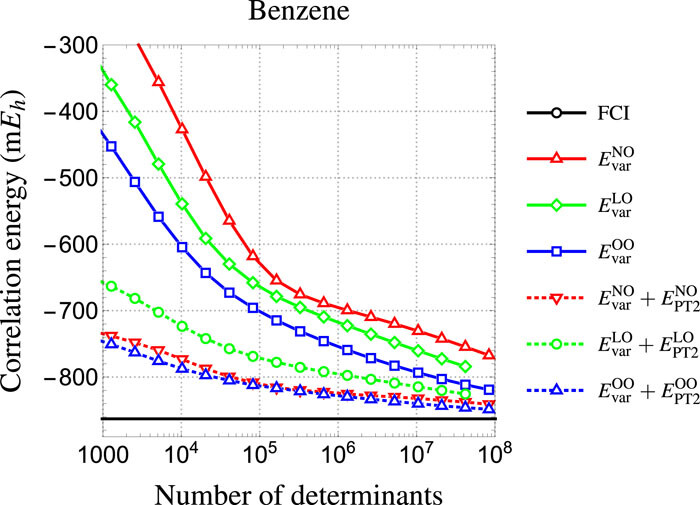
\includegraphics[width=0.9\textwidth]{fig/oocipsi_benzene.jpeg}
                        \centering
                        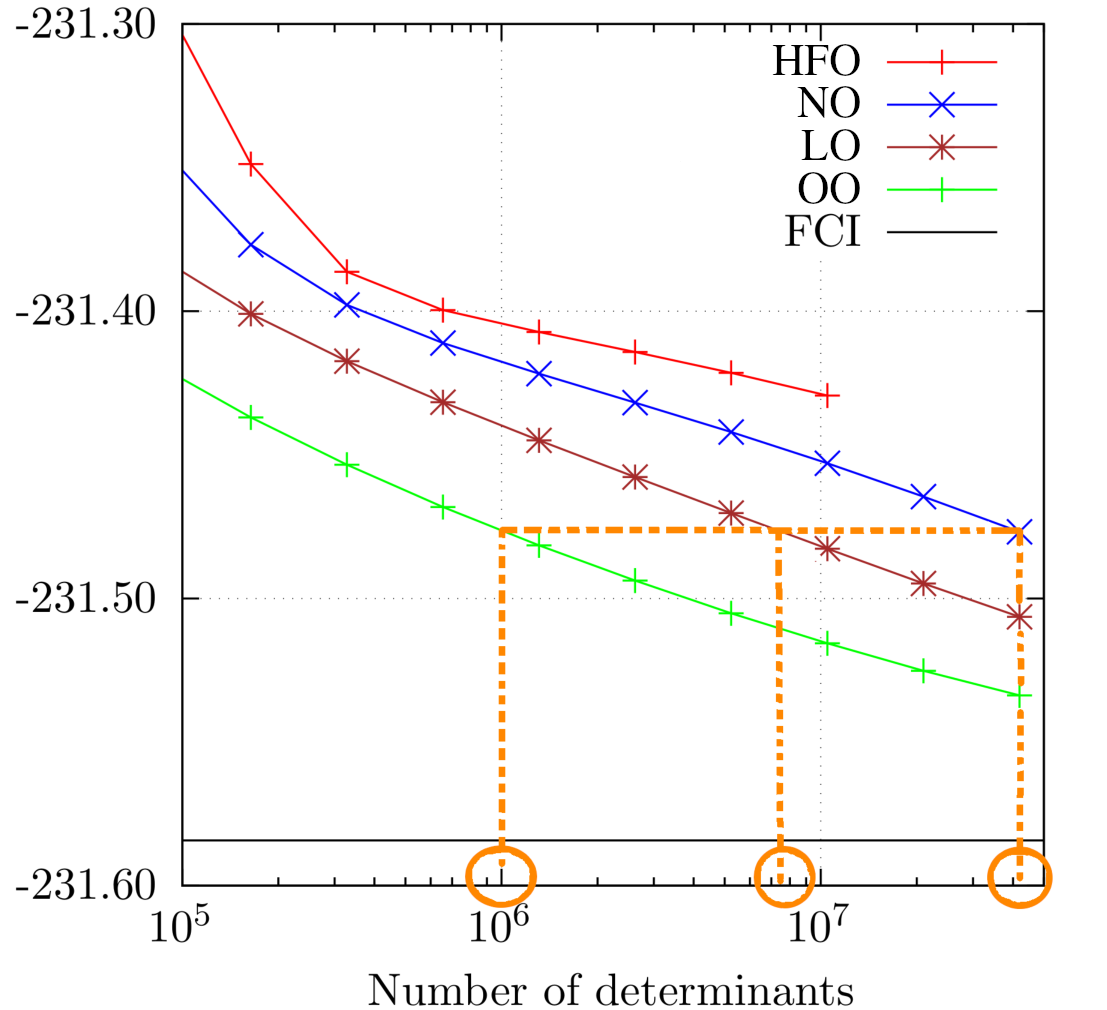
\includegraphics[width=0.8\textwidth]{fig/benzene.png}
                        %\\
                        %\bigskip
                        \end{block}
                \end{column}

        \end{columns}

                        \bigskip
                        \centering
	\url{https://github.com/Ydrnan/qp_plugins_damour/}

\end{frame}

\begin{frame}{Orbital optimized selected CI}

\begin{columns}

\begin{column}{0.5\textwidth}

\centering
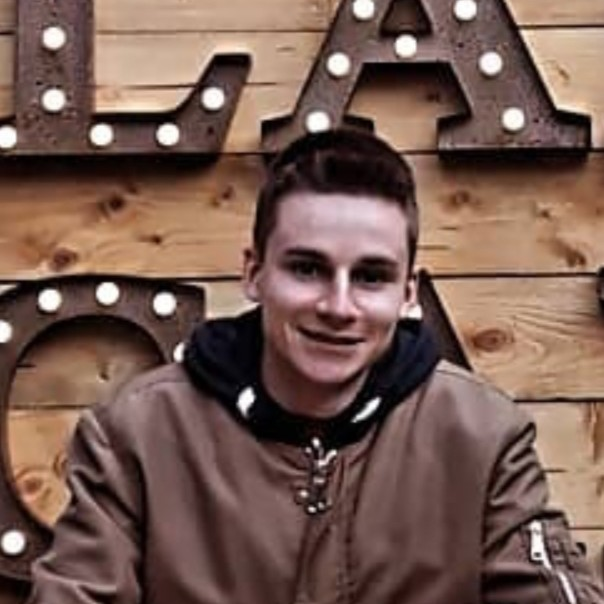
\includegraphics[width=0.4\textwidth]{fig/Yann2.jpg}
\\
Yann Damour
\\

\begin{itemize}
    \item Orbital optimization largely accelerates the convergence of selected CI
                        \bigskip
    \item Trust-region Newton-Raphson algorithm
                        \bigskip
\end{itemize}
            \bigskip
                        \centering
            \pub{JCP 155, 134104 (2021)}
\end{column}

                \begin{column}{0.5\textwidth}
                        \centering
            \begin{block}{Correlation energy for different sets of orbitals (Benzene / cc-pVDZ) }
                        %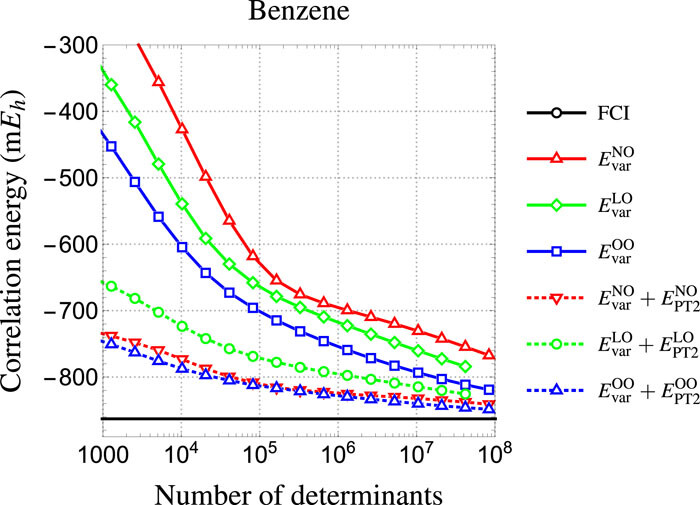
\includegraphics[width=0.9\textwidth]{fig/oocipsi_benzene.jpeg}
                        \centering
                        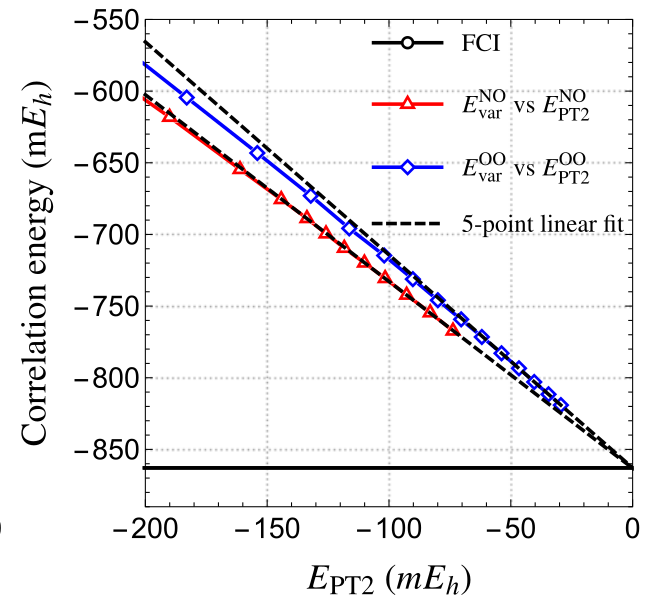
\includegraphics[width=0.8\textwidth]{fig/extrapolation.png}
                        %\\
                        %\bigskip
                        \end{block}
                \end{column}

        \end{columns}

                        \bigskip
                        \centering
    \url{https://github.com/Ydrnan/qp_plugins_damour/}

\end{frame}

%%%%%%%%%%%%%%%%%%%%%%%%%%%%%%%%%%%%%%%%%%%%


%%%%%%%%%%%%%%%%%%%%%%%%%%%%%%%%%%%%%%%%%%%%
\begin{frame}{Dipole moments and transition dipole moments}

\begin{columns}
\begin{column}{0.5\textwidth}

\centering
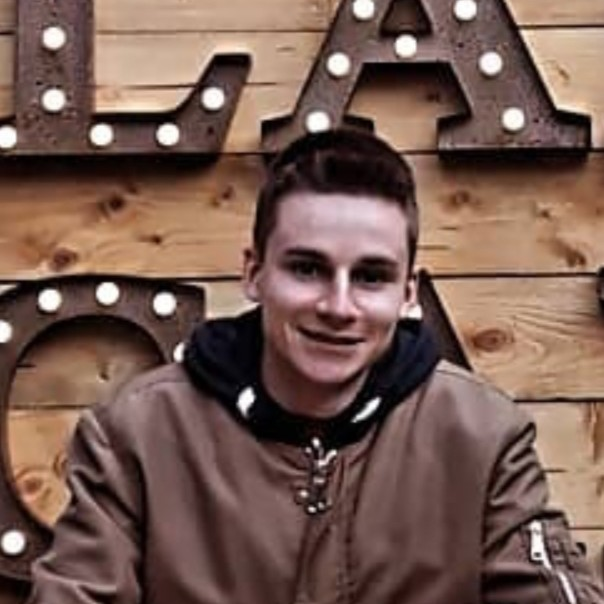
\includegraphics[width=0.4\textwidth]{fig/Yann2.jpg}
\\
Yann Damour
\\
\begin{itemize}

	\item UV/Vis spectroscopy
                        \bigskip
	\item Challenging for theory: \\ largely dependent on method and basis set 
                        \bigskip
	\item Selected CI approach 
\end{itemize}
\end{column}

                \begin{column}{0.5\textwidth}
                        \centering
                        \begin{block}{2nd excited state of \ce{H2S}/AVTZ}
			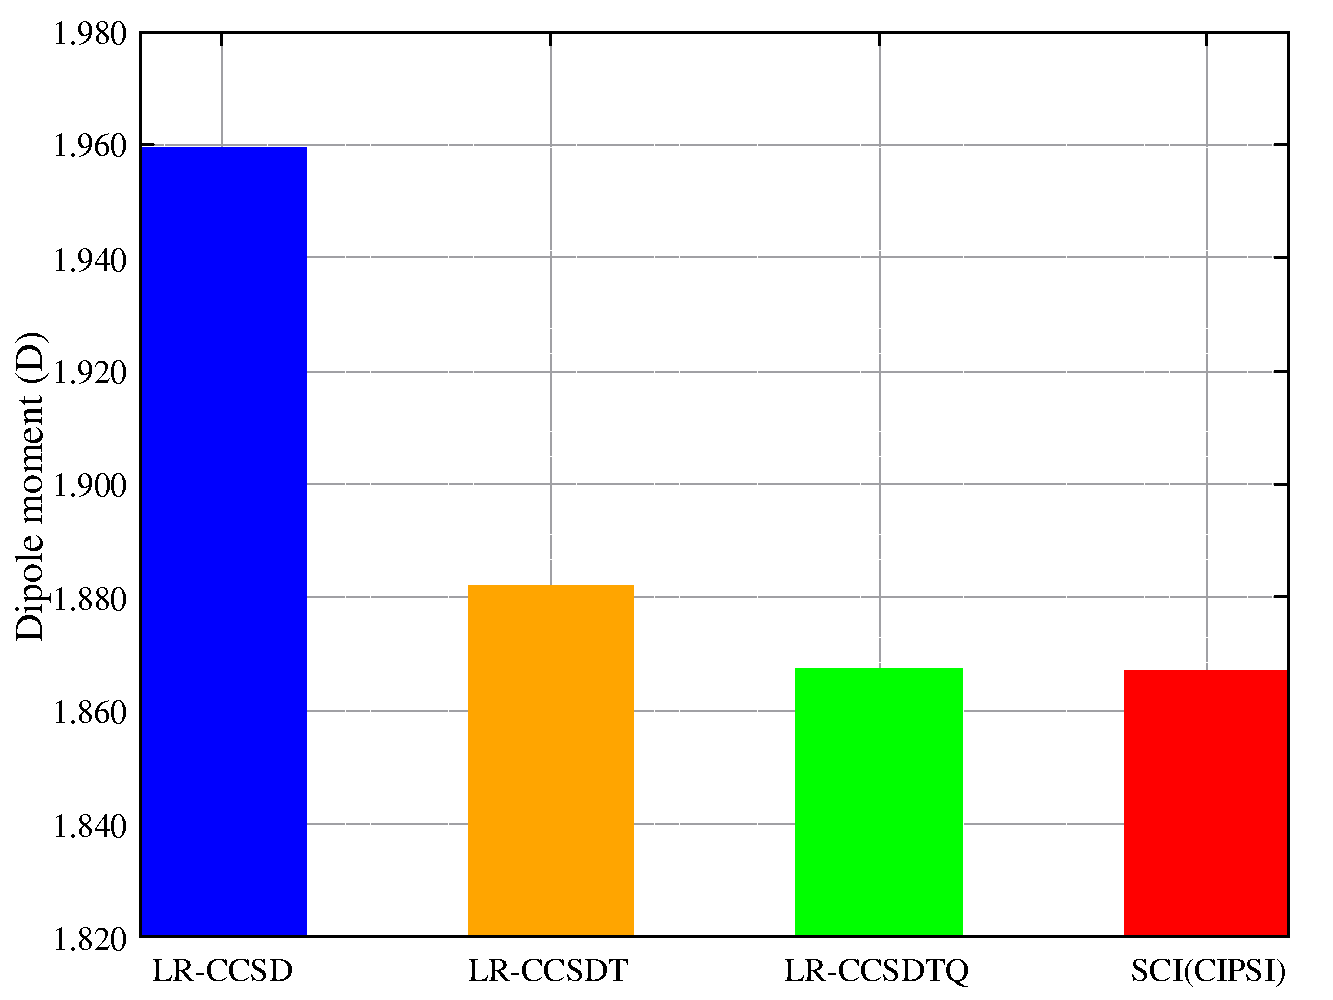
\includegraphics[width=1.0\textwidth]{fig/h2s_avtz.pdf}
                        \end{block}
                \end{column}

        \end{columns}

                        \bigskip
                        \centering
        \url{https://github.com/Ydrnan/qp_plugins_damour/}

\end{frame}
%%%%%%%%%%%%%%%%%%%%%%%%%%%%%%%%%%%%%%%%%%%%


%%%%%%%%%%%%%%%%%%%%%%%%%%%%%%%%%%%%%%%%%%%%
\begin{frame}{Many-Body Perturbation Theory}

        \begin{columns}
                \begin{column}{0.55\textwidth}
                        \centering
                        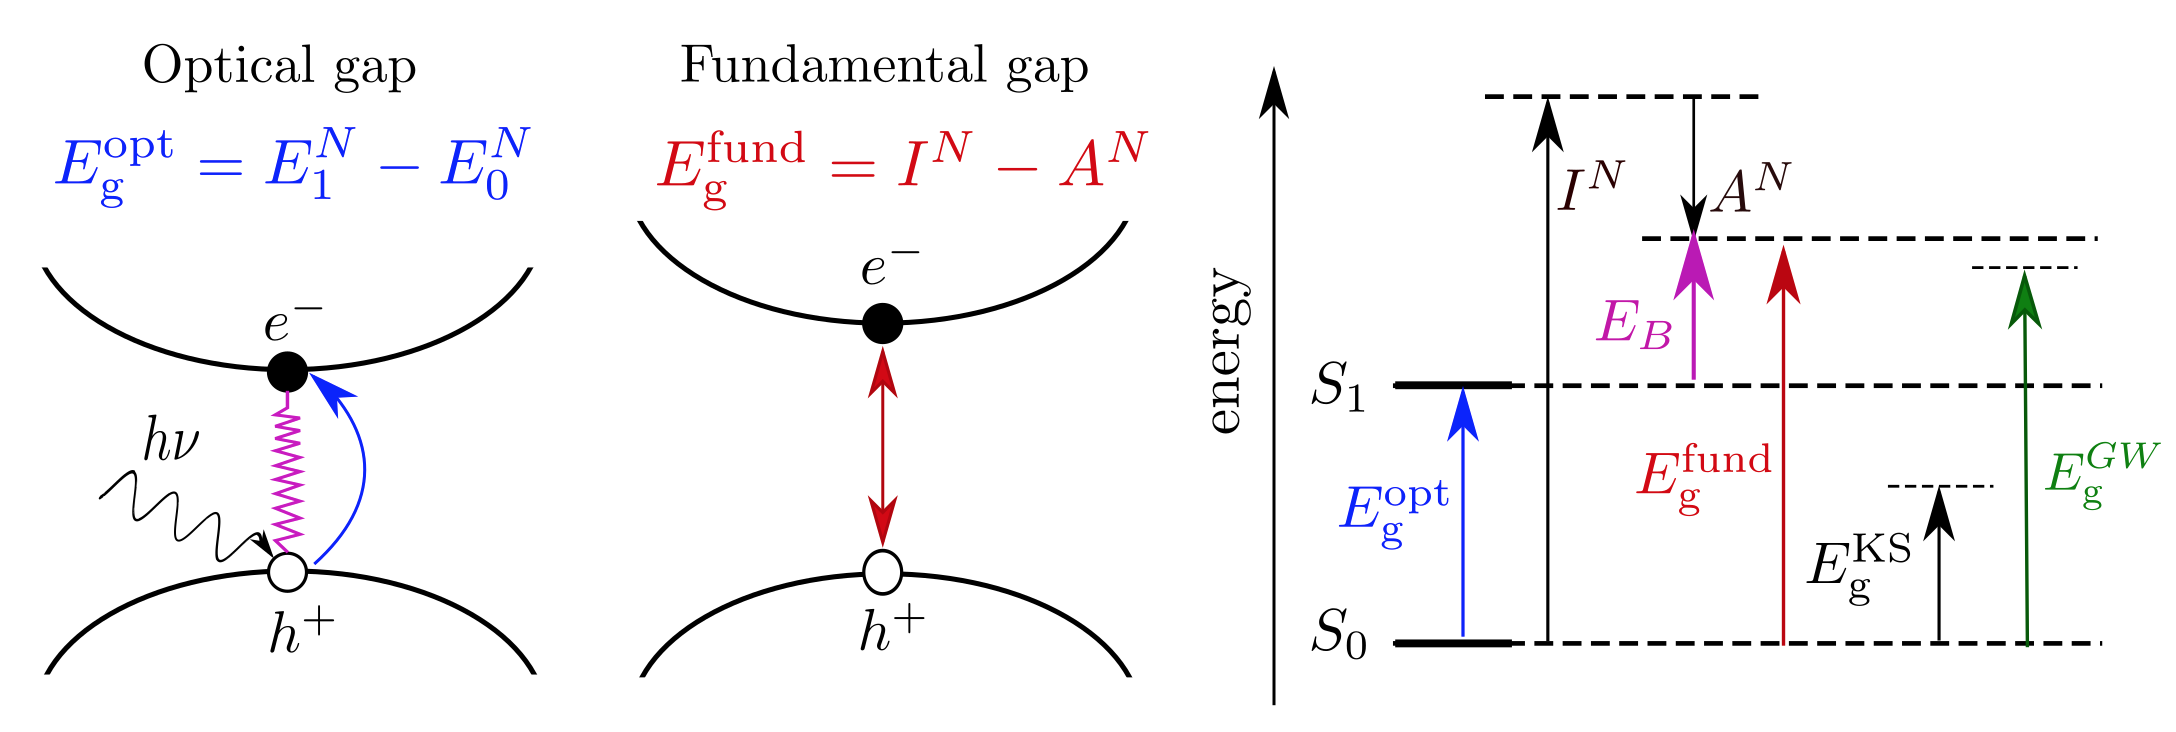
\includegraphics[width=1.05\textwidth]{fig/gaps}
                \end{column}
                \begin{column}{0.45\textwidth}
                        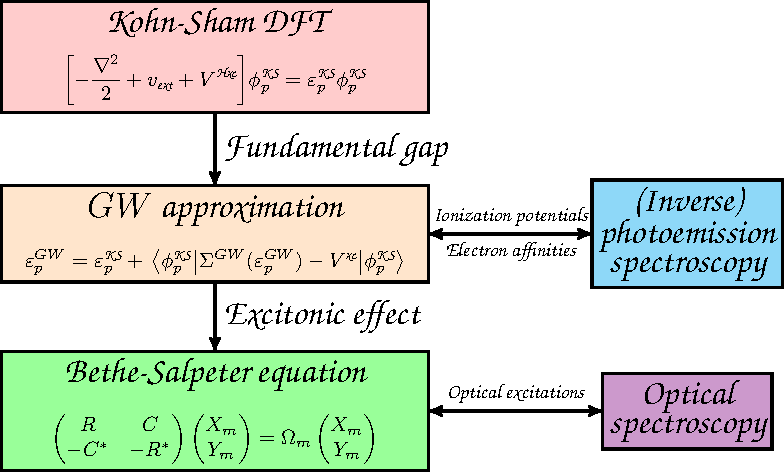
\includegraphics[width=1.00\textwidth]{fig/TOC_BSE-GW}
                \end{column}
        \end{columns}

        \begin{columns}
                \begin{column}{0.25\textwidth}
\centering
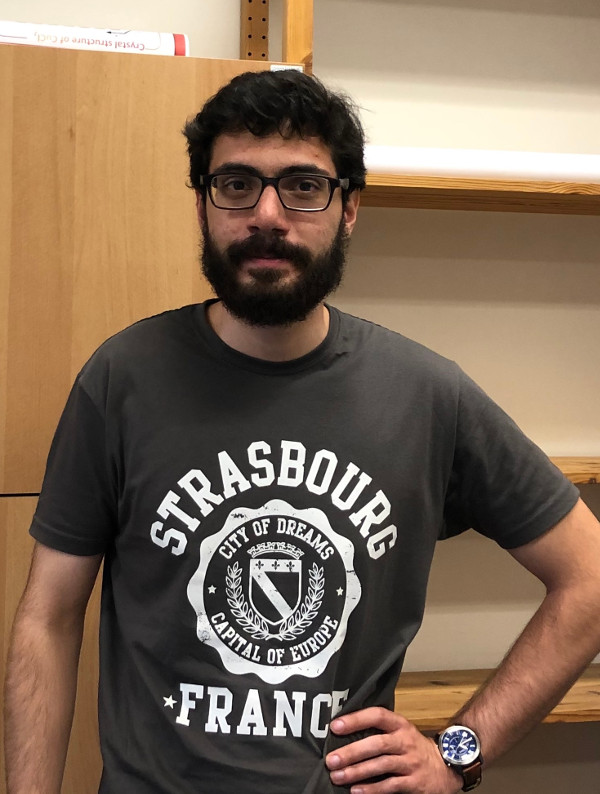
\includegraphics[width=0.6\textwidth]{fig/Roberto}
\\
Roberto Orlando
                \end{column}
                \begin{column}{0.25\textwidth}
\centering
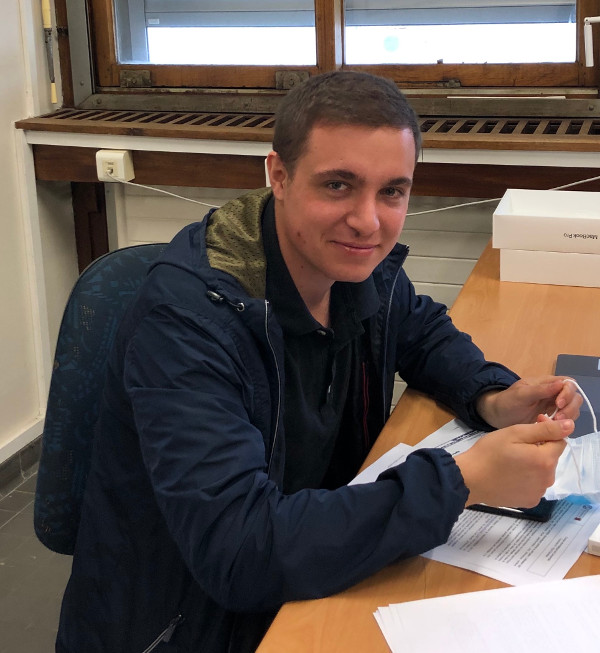
\includegraphics[width=0.7\textwidth]{fig/Enzo}
\\
Enzo Monino
                \end{column}

                \begin{column}{0.50\textwidth}
		\begin{itemize}
			\item Regularization in $GW$ Methods
		\end{itemize}
		\pub{Monino \& Loos, arxiv (2022)}
                \end{column}
                \end{columns}

\end{frame}
%%%%%%%%%%%%%%%%%%%%%%%%%%%%%%%%%%%%%%%%%%%%


%%%%%%%%%%%%%%%%%%%%%%%%%%%%%%%%%%%%%%%%%%%%
\begin{frame}{Many-Body Perturbation Theory}
        \begin{columns}
                \begin{column}{0.4\textwidth}
                        \centering
                        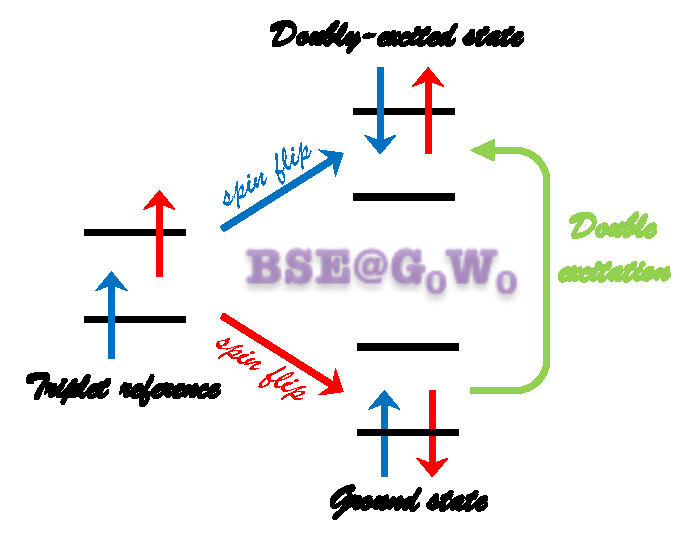
\includegraphics[width=0.90\textwidth]{fig/spin_flip_BSE_TOC.pdf}
                \end{column}
                \begin{column}{0.6\textwidth}
                        \centering
                        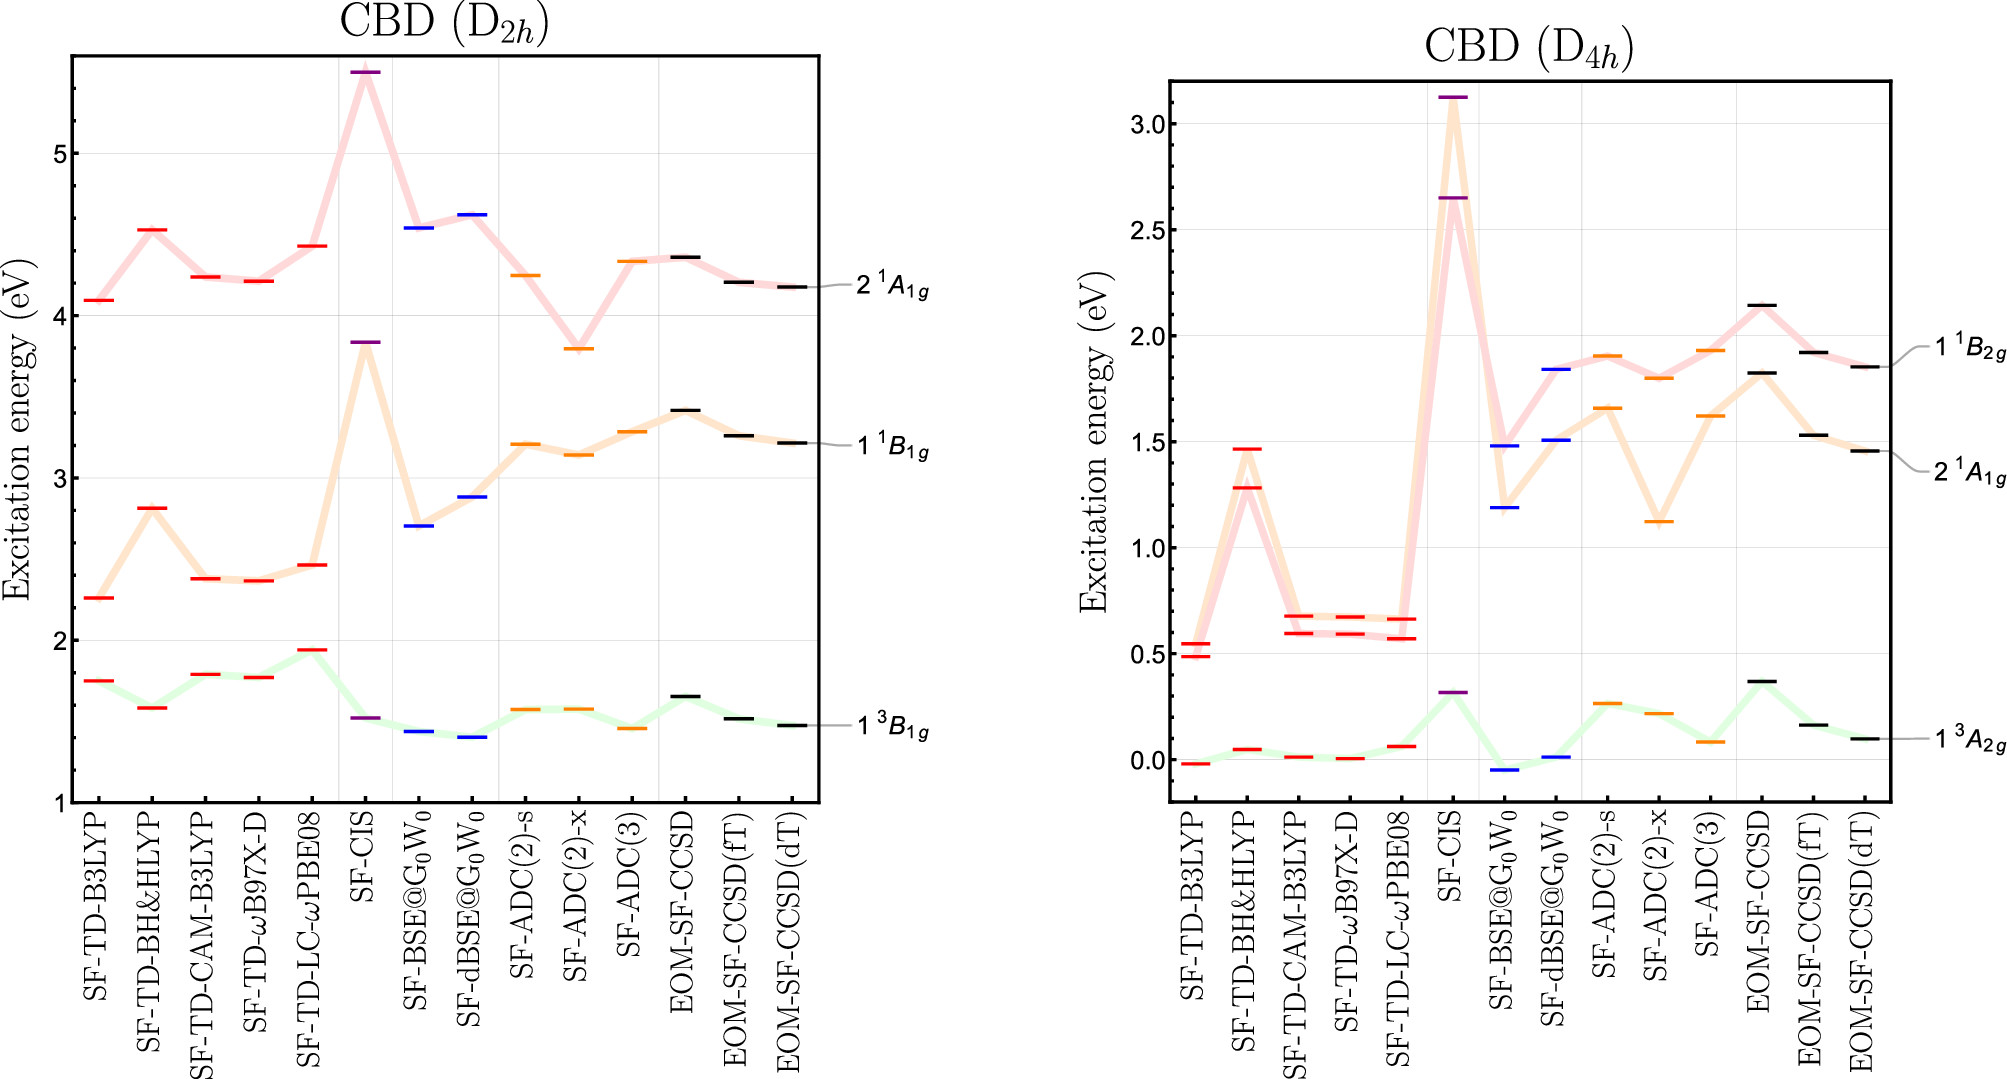
\includegraphics[width=0.95\textwidth]{fig/CDB_Enzo.jpeg}
                \end{column}
        \end{columns}
        \begin{columns}
        \begin{column}{0.50\textwidth}
\centering
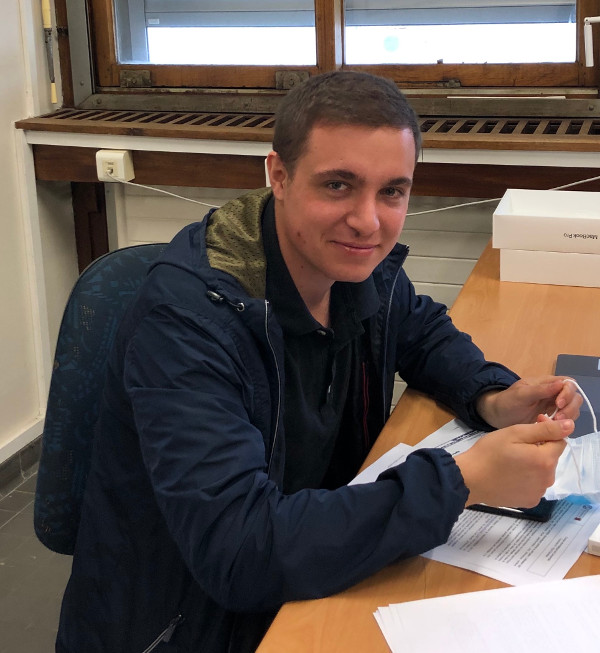
\includegraphics[width=0.35\textwidth]{fig/Enzo}
\\
Enzo Monino
        \end{column}

        \begin{column}{0.50\textwidth}
	\begin{itemize}
	\item Spin-Flip Bethe–Salpeter Equation Formalism
	\end{itemize}
	\pub{JCTC 17, 2852 (2021)}
        \end{column}
        \end{columns}
\end{frame}
%%%%%%%%%%%%%%%%%%%%%%%%%%%%%%%%%%%%%%%%%%%%


%%%%%%%%%%%%%%%%%%%%%%%%%%%%%%%%%%%%%%%%%%%%
\begin{frame}{Gross-Oliveira-Kohn (GOK) DFT for neutral excitations}
        \begin{columns}
        \begin{column}{0.80\textwidth}

        Ensemble energy:
        \begin{equation*}
                \boxed{E^{\bm{w}}= (1 - w_1 - w_2) E^{(0)} + w_1 E^{(1)} + w_2 E^{(2)}}
        \end{equation*}

        Excitation energies:
        \begin{equation*}
                \pdv{E^{\bm{w}}}{w_{1}}= E^{(1)} - E^{(0)} = \Omega^{(1)}
                \qquad \pdv{E^{\bm{w}}}{w_{2}}= E^{(2)} - E^{(0)} = \Omega^{(2)}
        \end{equation*}

        Ensemble energy in practice:
        \begin{equation*}
                E^{\bm{w}} = \min_{n} \qty{ \alert{F^{\bm{w}}[n]} + \int v_\text{ext}(\br{}) n(\br{}) d\br{} }
                \qquad
                \alert{F^{\bm{w}}[n]} = T_\text{s}^{\bm{w}}[n] + \purple{E_\text{Hxc}^{\bm{w}}[n]}
        \end{equation*}

        Derivative discontinuity:
        \begin{equation*}
                \boxed{
                \pdv{E^{\bm{w}}}{w_I}
                = \mathcal{E}_{I}^{\bm{w}} - \mathcal{E}_{0}^{\bm{w}}
                + \left. \pdv{\purple{E_\text{xc}^{\bm{w}}[n]}}{w_{I}} \right|_{n = n^{\bm{w}}(\br{})}
                \qquad
                \purple{E_\text{xc}^{\bm{w}}[n]} = \int \blue{\epsilon_\text{xc}^{\bm{w}}(n(\br{}))} n(\br{}) d\br{}
                }
        \end{equation*}

        \end{column}

        \begin{column}{0.25\textwidth}
\centering
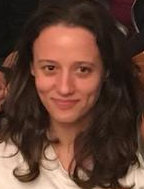
\includegraphics[width=0.6\textwidth]{fig/Clotilde}
\\
Clotilde Marut
\bigskip

	\begin{itemize}
	\item Construction of weight-dependent exchange–correlation functionals

	\pub{Faraday Discuss. 224, 4023 (2020)}
	\end{itemize}
        \end{column}
        \end{columns}

\end{frame}
%%%%%%%%%%%%%%%%%%%%%%%%%%%%%%%%%%%%%%%%%%%%


%%%%%%%%%%%%%%%%%%%%%%%%%%%%%%%%%%%%%%%%%%%%
\begin{frame}{Ensemble DFT for charged excitations}
        \begin{columns}
                \begin{column}{0.80\textwidth}
		\begin{block}{PPLB formalism (fractional electrons)}
		\pub{Perdew, Parr, Levy \& Balduz PRL 49, 1691 (1982)}
        \begin{align*}
                E^{\bm{\alpha}} & = \qty(1 - \alpha_1 - \alpha_2) E^{N} + \alpha_1 E^{N-1} + \alpha_2 E^{N+1}
                        \\
                n^{\bm{\alpha}} & = \qty(1 - \alpha_1 - \alpha_2) n^{N} + \alpha_1 \Gamma^{N-1} + \alpha_2 n^{N+1}
                        \qq{$\Rightarrow$} \red{\int n^{\bm{\alpha}} d\br{} = N - \alpha_1 + \alpha_2}
                        \\
                        & \qq{$\Rightarrow$ \red{The exact xc functional does not need to be weight-dependent}}
        \end{align*}

        \end{block}
		\begin{block}{$N$-centered formalism}
		\pub{Senjean \& Fromager PRA 98, 022513 (2018)}
        \begin{align*}
                E^{\bm{\xi}} & = \qty(1 - \frac{N-1}{N} \xi_1 - \frac{N+1}{N} \xi_2) E^{N} + \xi_1 E^{N-1} + \xi_2 E^{N+1}
                \\
                        n^{\bm{\alpha}} & = \qty(1 - \frac{N-1}{N} \xi_1 - \frac{N+1}{N} \xi_2) n^{N} + \xi_1 n^{N-1} + \xi_2 n^{N+1}
                        \qq{$\Rightarrow$} \green{\int n^{\bm{\xi}} d\br{} = N}
                        \\
                        & \qq{$\Rightarrow$ \green{The exact xc functional must be weight-dependent}}
        \end{align*}
        \end{block}
        \end{column}

        \begin{column}{0.25\textwidth}
\centering
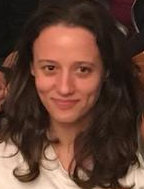
\includegraphics[width=0.6\textwidth]{fig/Clotilde}
\\
Clotilde Marut
        \end{column}
        \end{columns}

\end{frame}
%%%%%%%%%%%%%%%%%%%%%%%%%%%%%%%%%%%%%%%%%%%%


%%%%%%%%%%%%%%%%%%%%%%%%%%%%%%%%%%%%%%%%%%%%
\begin{frame}
\frametitle{Fock Space Coupled Cluster}

        \begin{columns}
        \begin{column}{0.80\textwidth}

\begin{block}{Fock-Space Coupled Cluster (FSCC)}

\begin{itemize}
\item FSCC describes both neutral and charged excitations

\item Fock space for a system of $n$ electrons and $m$  spin orbitals:

neutral (green), electron-detached (red), and electron-attached (blue) sectors 

\end{itemize}

\vspace{-0.5cm}
\begin{center}
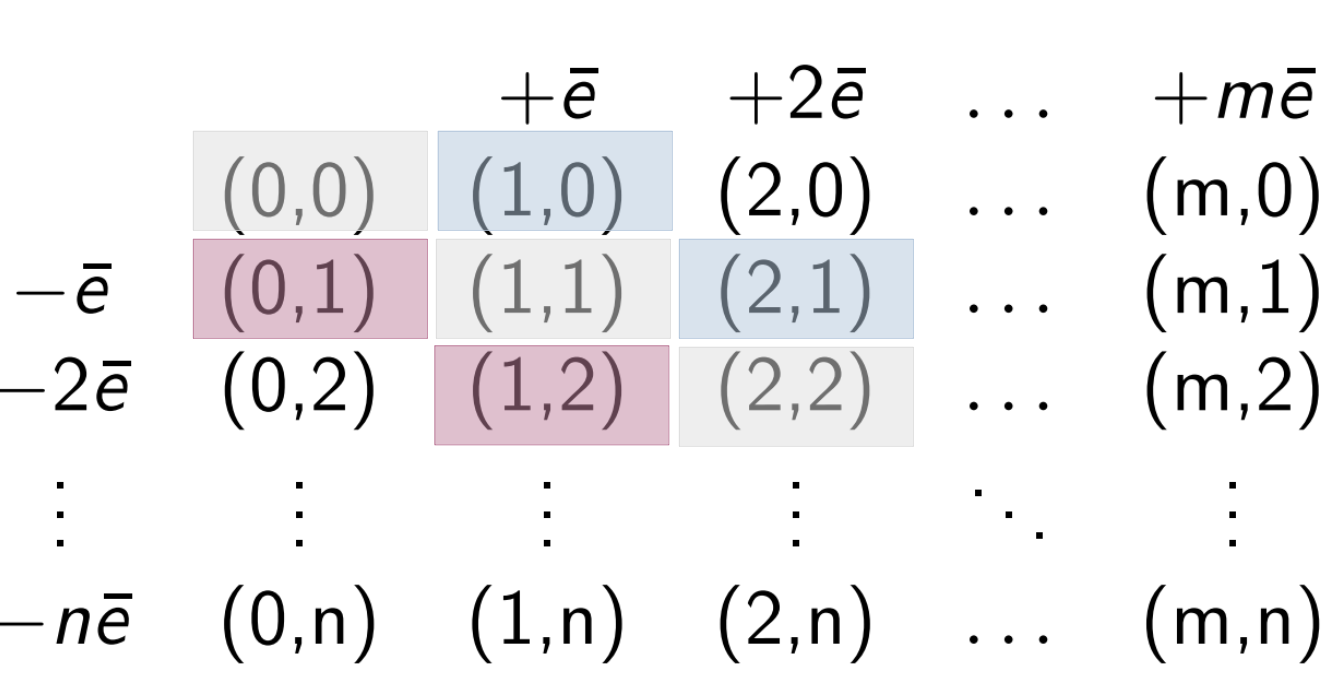
\includegraphics[width=0.4\textwidth]{fig/fscc.png}
\end{center}

\end{block}

\begin{block}{Goals}
\begin{itemize}
\item Generate the FSCC equations by using symbolic programming
\item Describe satellite (or shake-up) transitions
\end{itemize}
\end{block}
        \end{column}

        \begin{column}{0.20\textwidth}
\centering
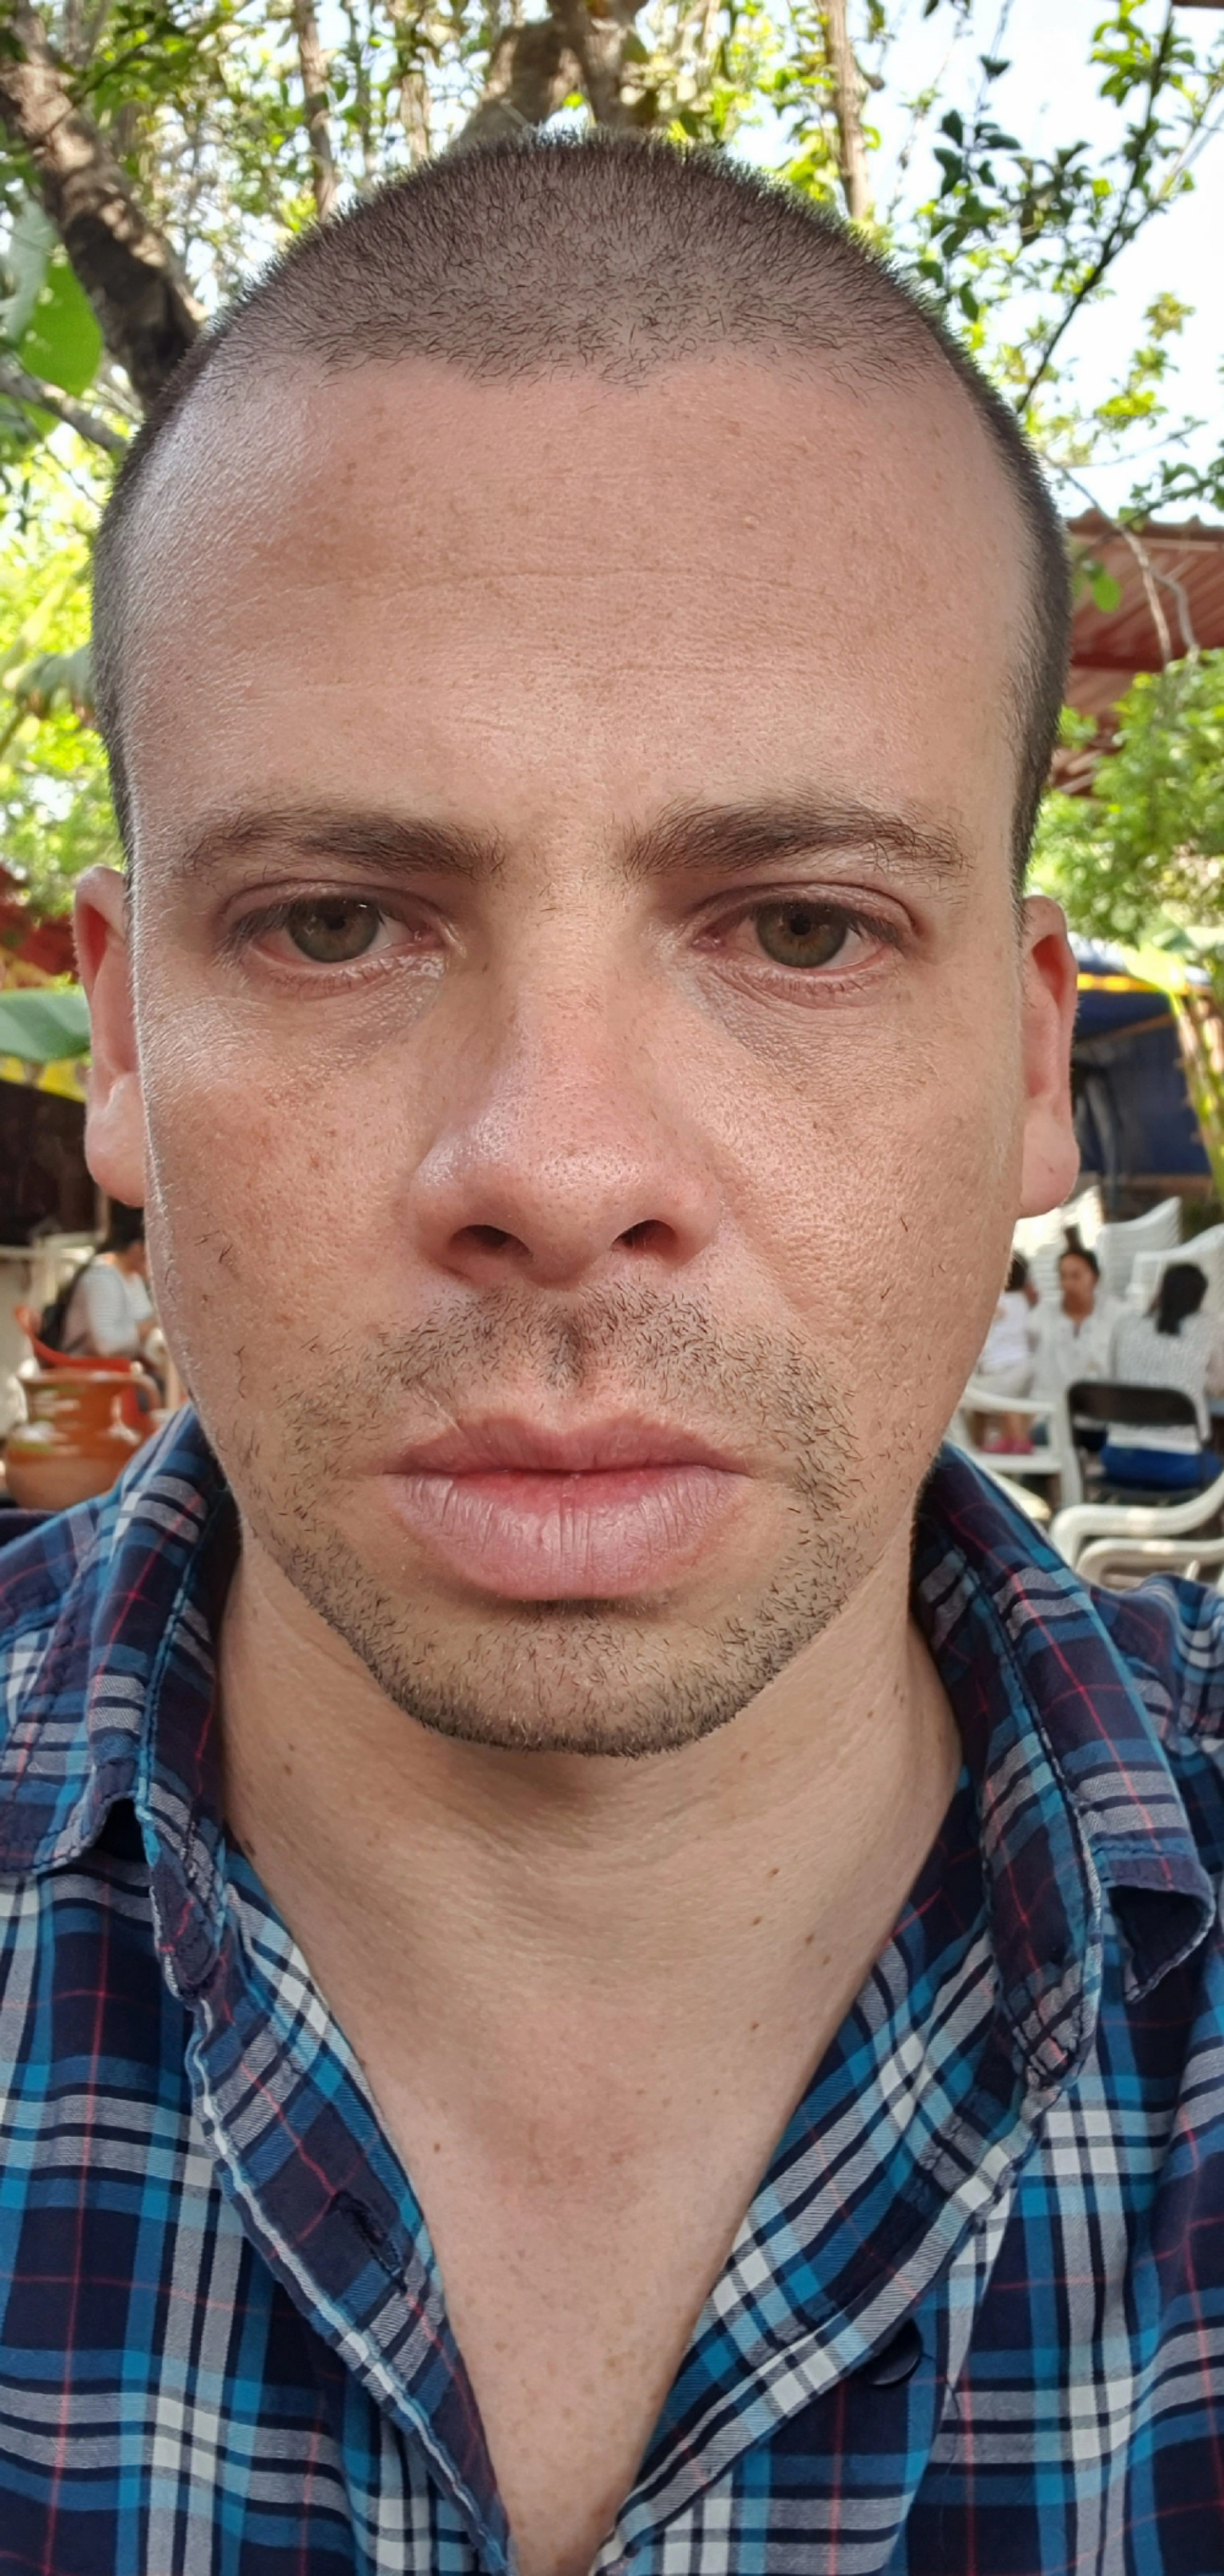
\includegraphics[width=0.6\textwidth]{fig/Raul.jpg}
\\
Raul Quintero
        \end{column}
        \end{columns}

\end{frame}
%%%%%%%%%%%%%%%%%%%%%%%%%%%%%%%%%%%%%%%%%%%%


%%%%%%%%%%%%%%%%%%%%%%%%%%%%%%%%%%%%%%%%%%%%
\begin{frame}
\frametitle{Fock Space Coupled Cluster}

        \begin{columns}
        \begin{column}{0.80\textwidth}
\begin{itemize}
\item 
Hole and particle operators:
\vspace{3mm}
\[
\hat{H}_{1}= \sum_{i}h_{i} \{\hat{i}\},\hspace{5mm} \hat{H}_{2}= \sum_{a,ij}h^{a}_{ij} \{\hat{a}^{\dagger}\hat{i}\hat{j}\},\hspace{5mm}\hat{P}_{1}= \sum_{a}p^{a}\{\hat{a}^{\dagger}\}, \hspace{5mm} \hat{P}_{2}= \sum_{ab,i}p^{ab}_{i} \{\hat{a}^{\dagger}\hat{b}^{\dagger}\hat{i}\}
\]
where  $h_{i}$ and $h^{a}_{ij}$ are ionization amplitudes, \\ while $p^{a}$ and $p^{ab}_{i}$ are electron-attached amplitudes

\item 
Important commutators:
\[
\left[ \hat{T}_{m},\hat{H}_{n} \right]=0, \hspace{20mm} \left[ \hat{T}_{m},\hat{P}_{n} \right]=0
\]
\[
\left[ \hat{P}_{m},\hat{H}_{n} \right] \neq 0 \hspace{10mm}   \left[ \hat{P}_{m},\hat{P}_{n} \right] \neq 0 \hspace{10mm}   \left[ \hat{H}_{m},\hat{H}_{n} \right] \neq 0
\]

Excitation and charge operators commute; \\ charge operators do not commute among themselves

\item 
We target two diagonals of the Fock Space: \\ the main diagonal and one representing a charged excitation
\end{itemize}
        \end{column}

        \begin{column}{0.20\textwidth}
\centering
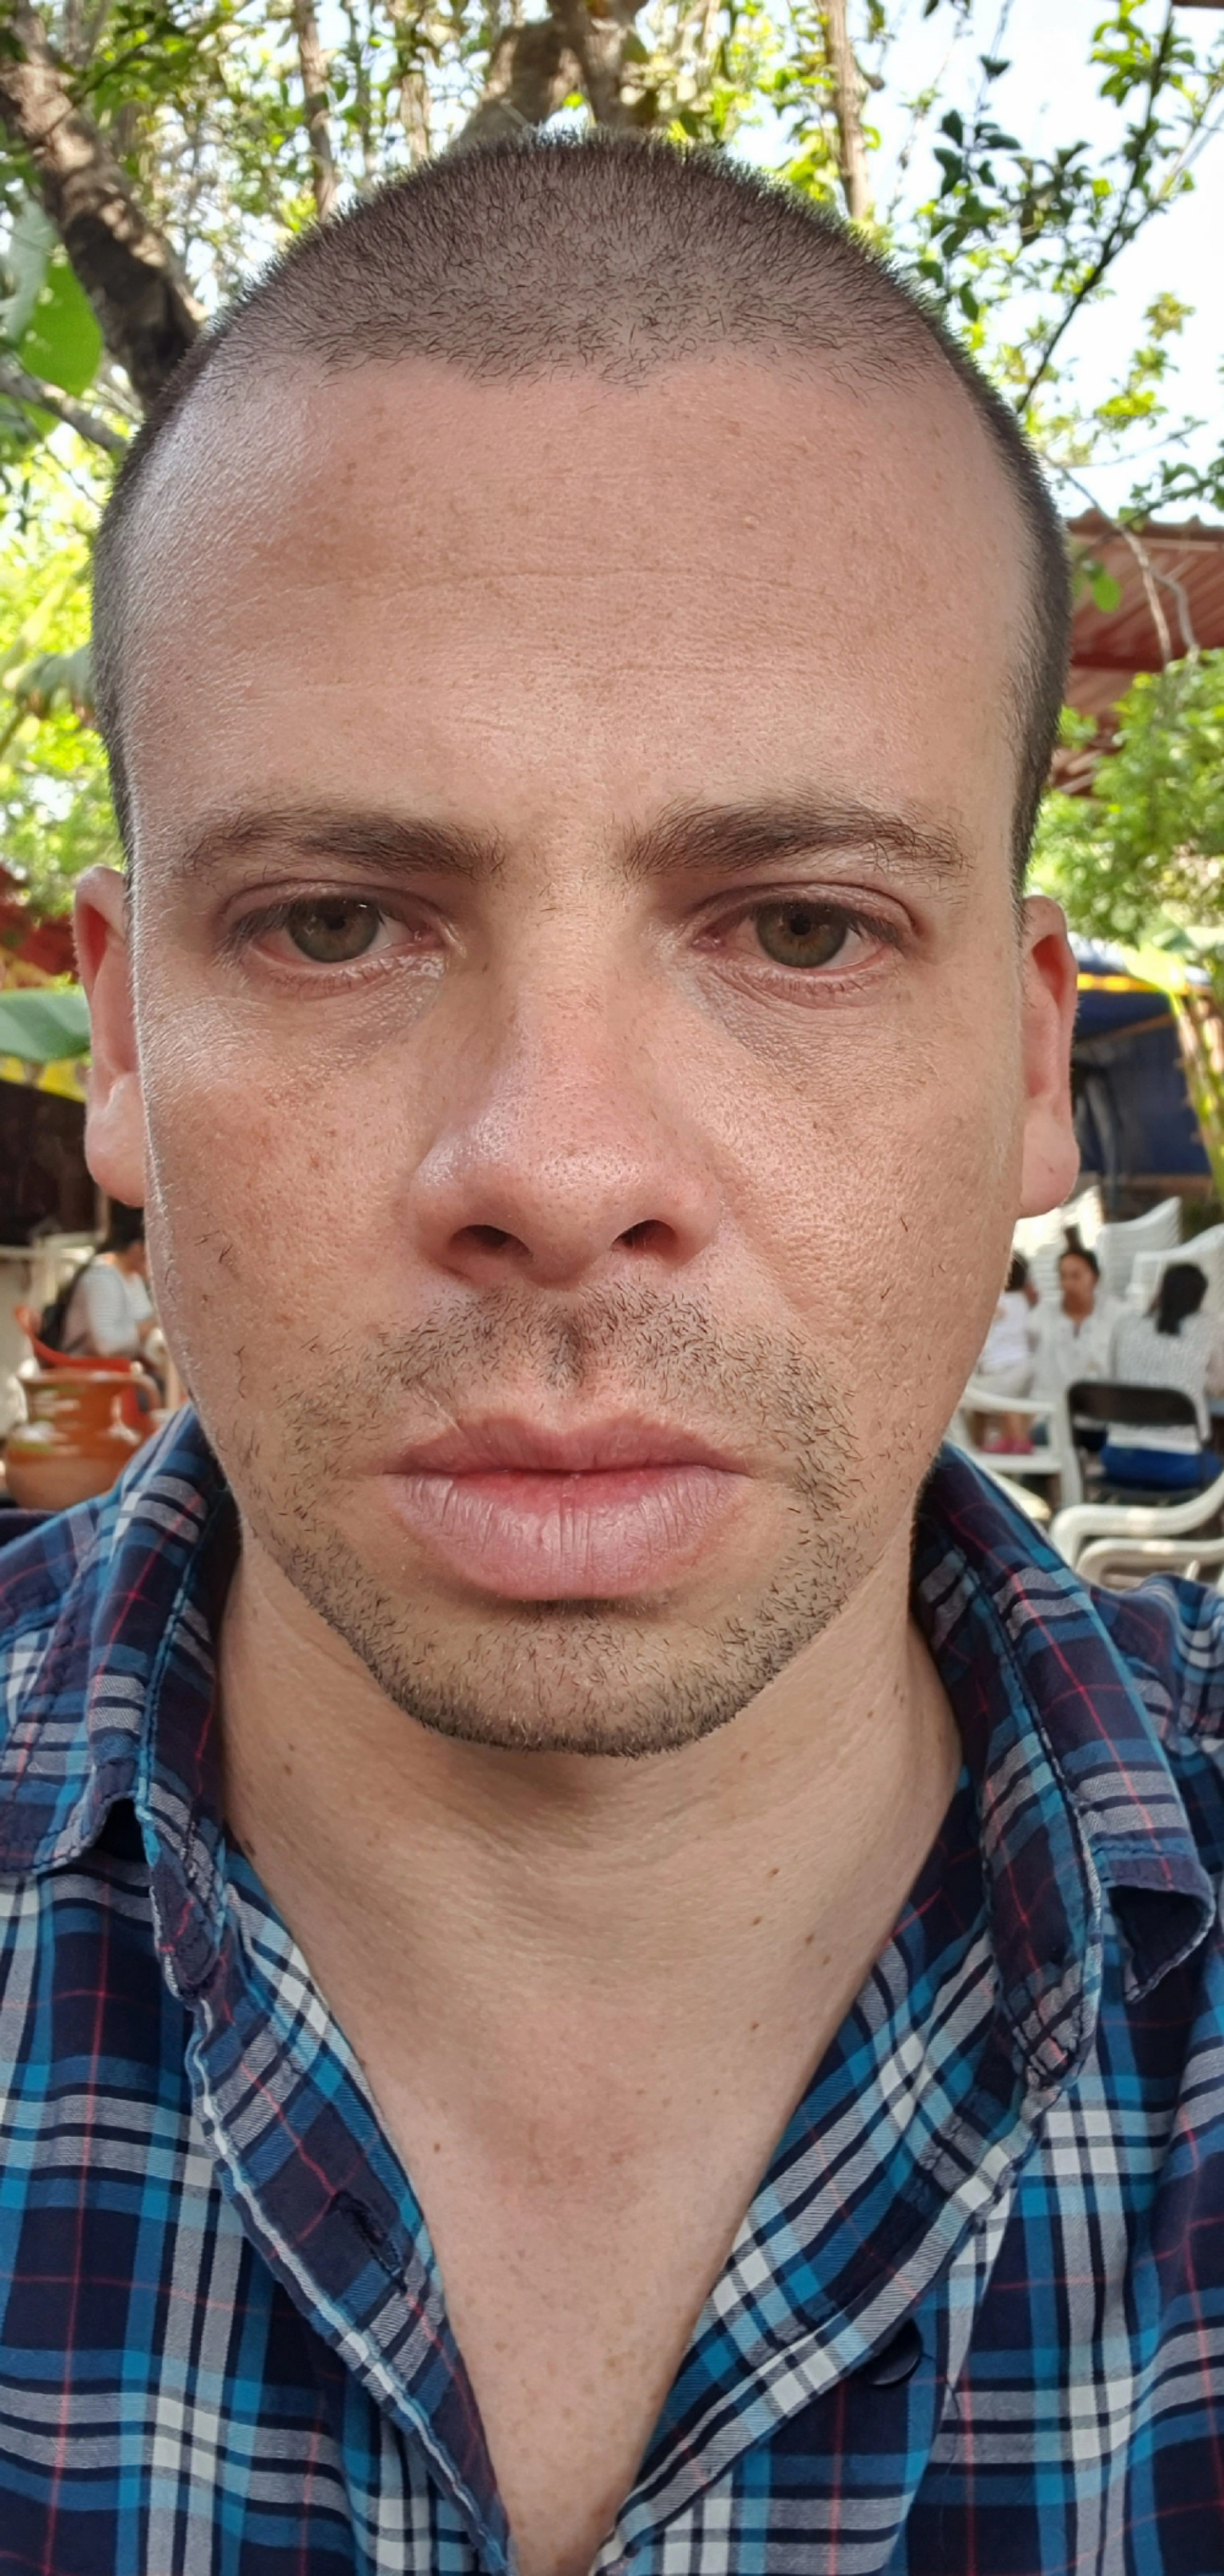
\includegraphics[width=0.6\textwidth]{fig/Raul.jpg}
\\
Raul Quintero
        \end{column}
        \end{columns}

\end{frame}
%%%%%%%%%%%%%%%%%%%%%%%%%%%%%%%%%%%%%%%%%%%%


%%%%%%%%%%%%%%%%%%%%%%%%%%%%%%%%%%%%%%%%%%%%
\begin{frame}{Coupled-Cluster for Excited States}

                \begin{columns}
                \begin{column}{0.25\textwidth}
			\centering
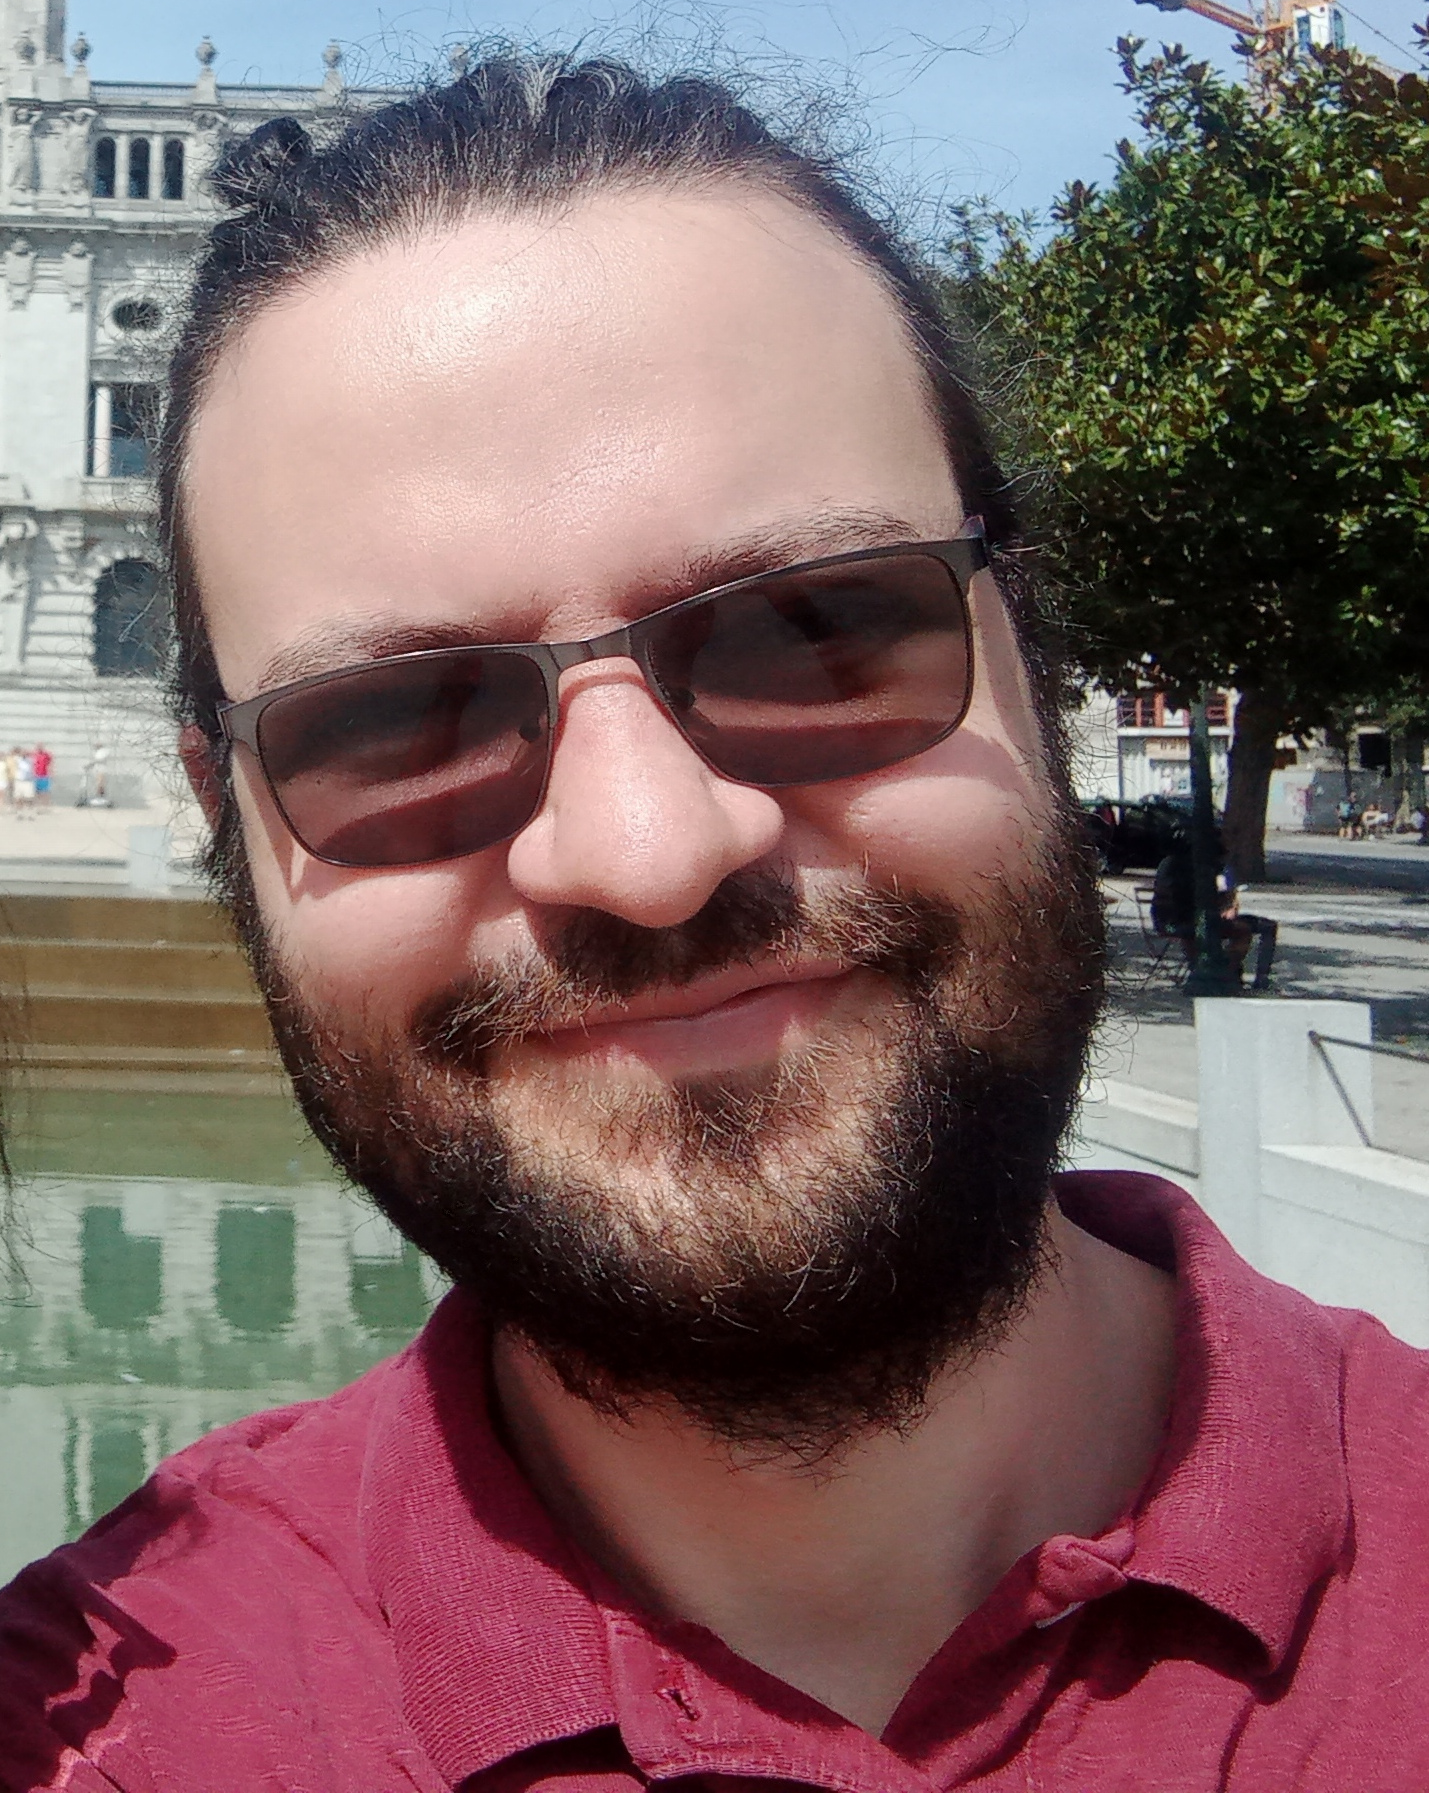
\includegraphics[width=0.6\textwidth]{fig/Fabris_2021.png}
\\
Fábris Kossoski
\bigskip

			\centering
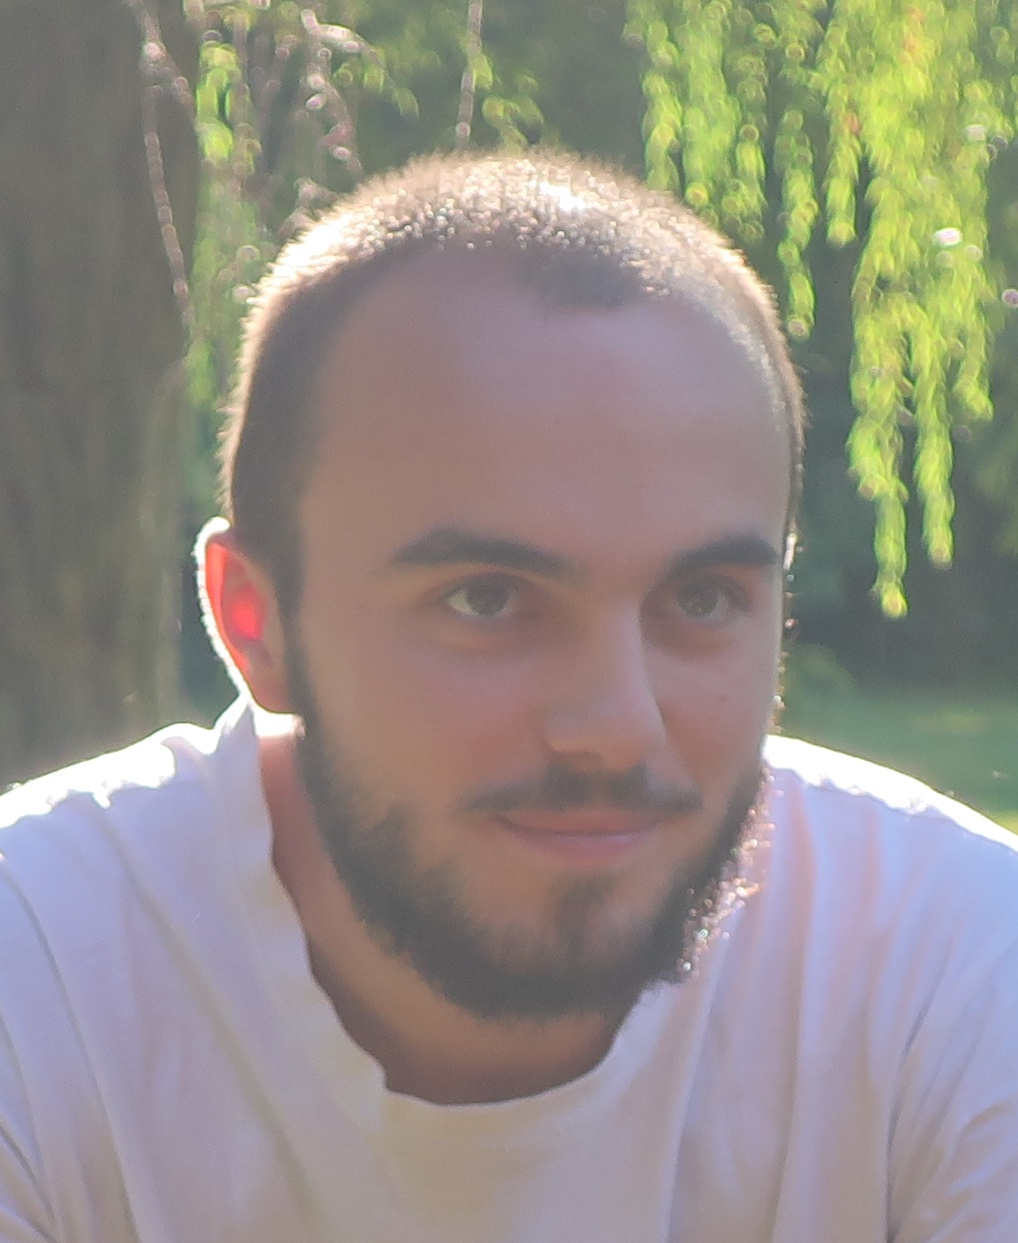
\includegraphics[width=0.6\textwidth]{fig/Antoine.jpg}
\\
Antoine Marie

                \end{column}

                \begin{column}{0.35\textwidth}
		\pub{JCTC 17, 4756 (2021)}
%		\bigskip

		\pub{JCP 155, 104105 (2021)}
                        \begin{block}{pCCD solutions for He/6-31G}
                                \centering
                                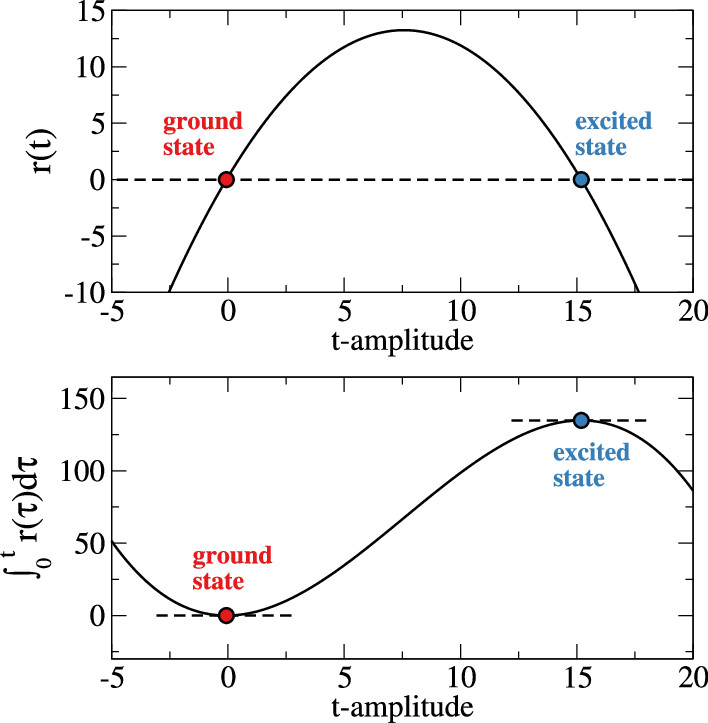
\includegraphics[width=\textwidth]{fig/scan_t}
                        \end{block}
                \end{column}
                \begin{column}{0.40\textwidth}
                        \centering
                        \begin{block}{pCCD vs DOCI for \ce{H4}/STO-6G}
                                \centering
                                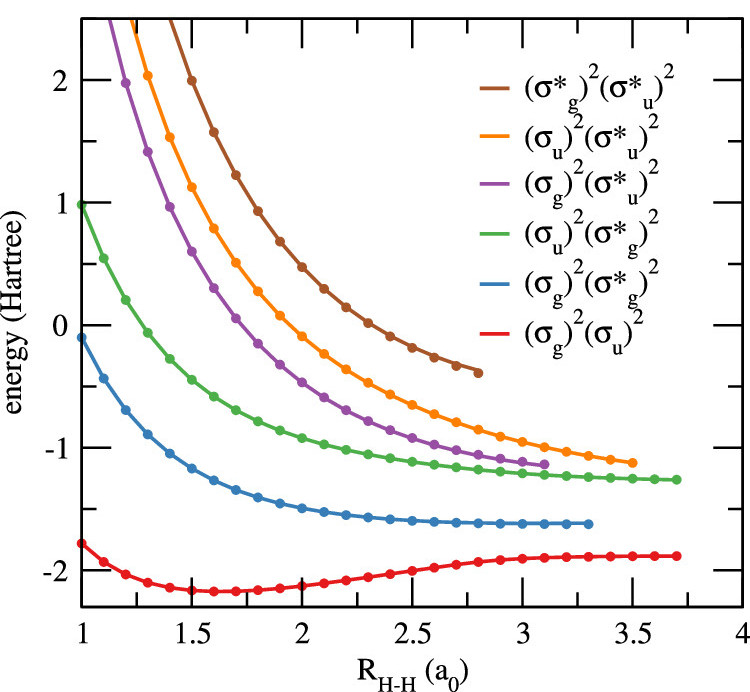
\includegraphics[width=0.8\textwidth]{fig/pccd.jpeg}
                        \end{block}
                \end{column}
        \end{columns}

\end{frame}
%%%%%%%%%%%%%%%%%%%%%%%%%%%%%%%%%%%%%%%%%%%%


%%%%%%%%%%%%%%%%%%%%%%%%%%%%%%%%%%%%%%%%%%%%
\begin{frame}{Hierarchy Configuration Interaction}

        \begin{columns}
        \begin{column}{0.25\textwidth}
        \centering
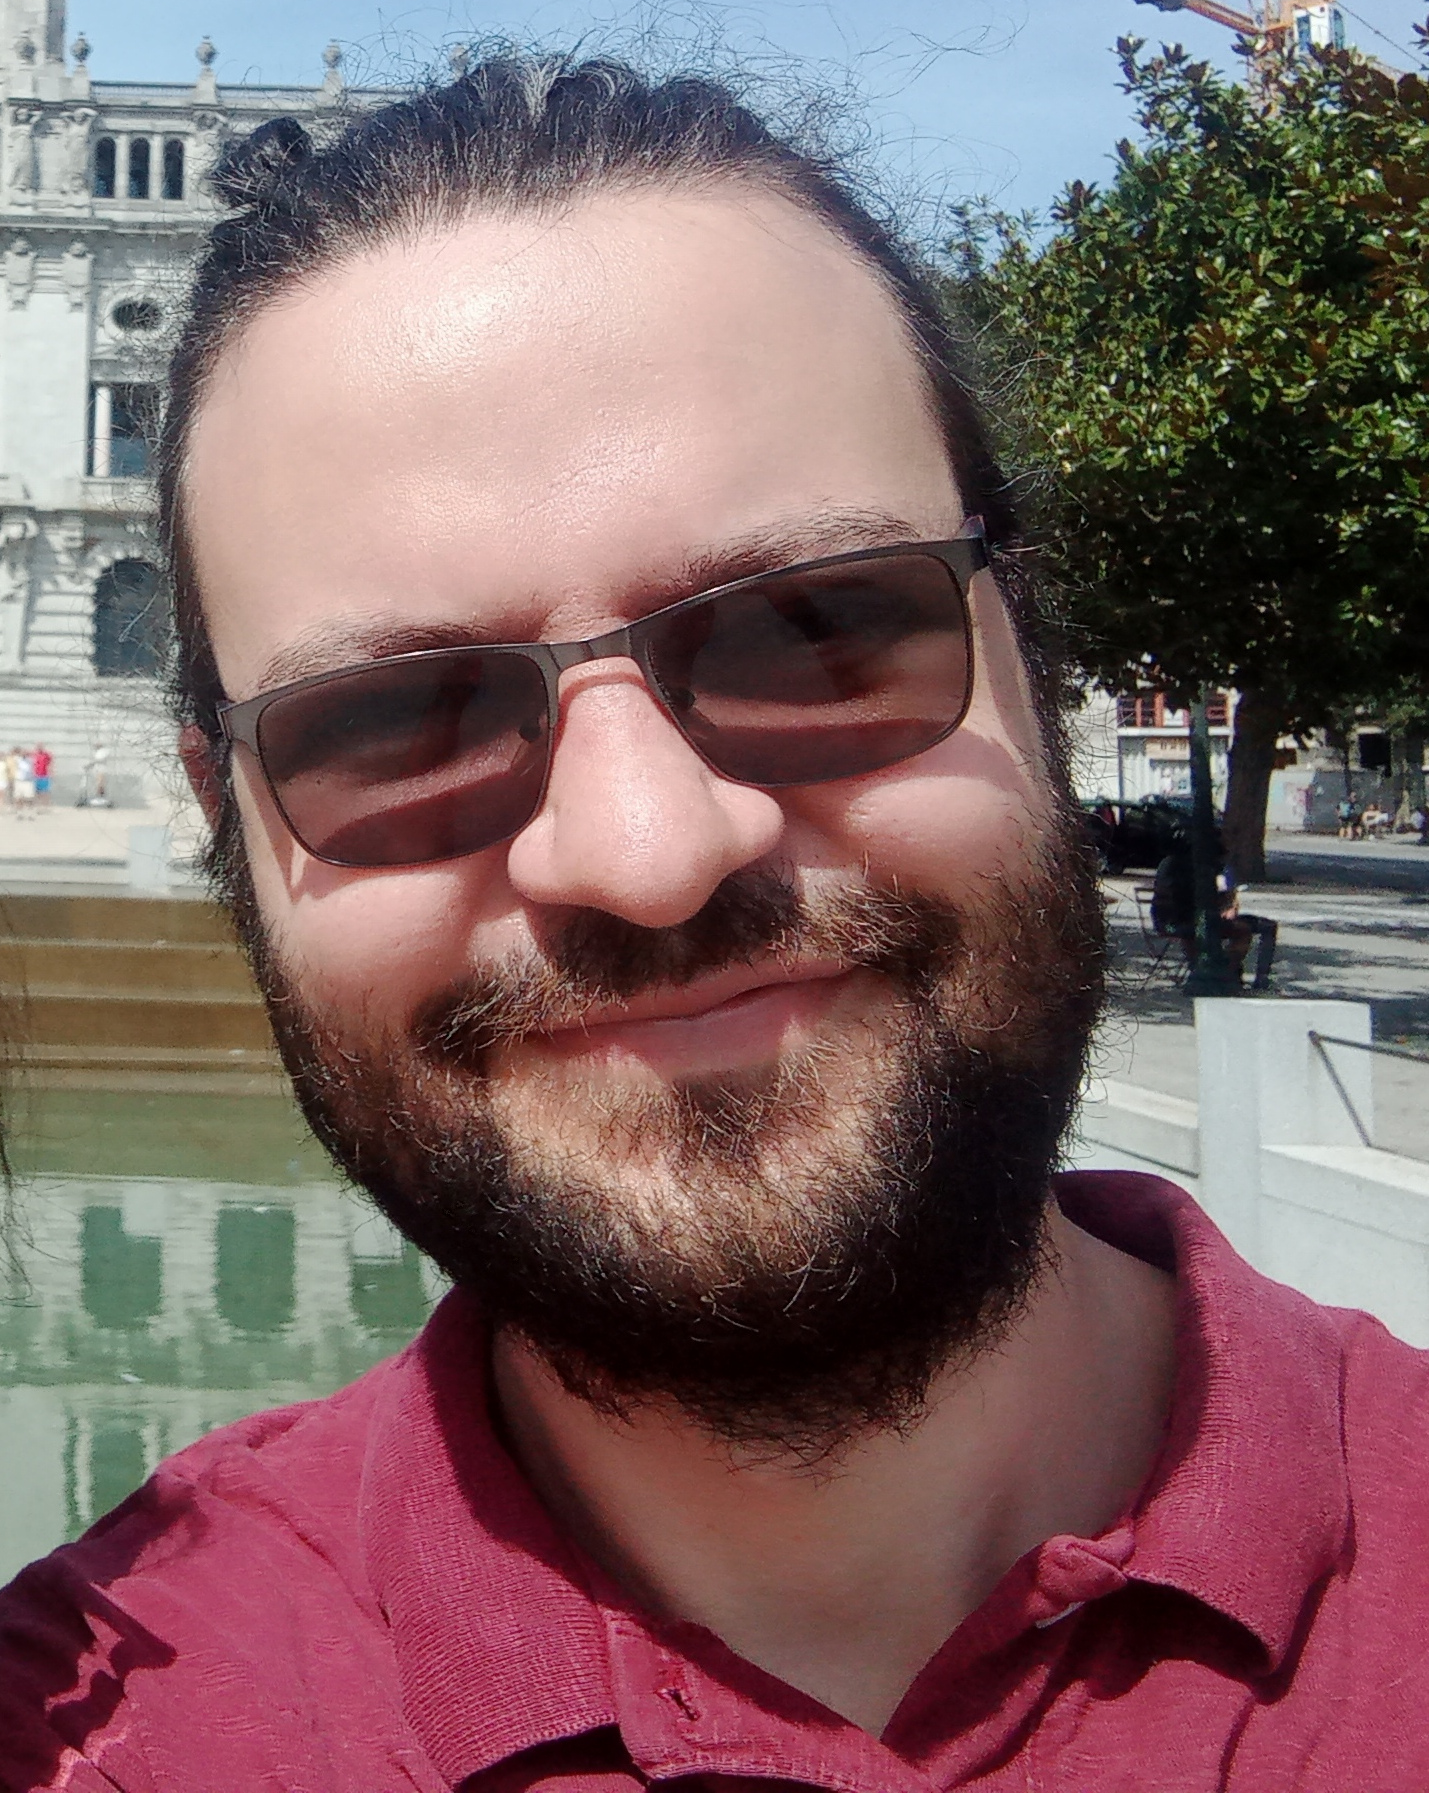
\includegraphics[width=0.6\textwidth]{fig/Fabris_2021.png}
\\
Fábris Kossoski
\\
\bigskip
        \centering
	\pub{JPCL 13, 4342 (2022)}
        \end{column}

        \begin{column}{0.35\textwidth}
	\smartdiagramset{
	font=\large,
	text width=4.5cm,
	set color list={green!10,green!00}}
	\smartdiagramset{module x sep = 6.2, back arrow disabled = true, uniform arrow color = true, arrow color = white}
	\smartdiagram[flow diagram:horizontal]{
	{\small Excitation degree $e$}\\
	{\small Seniority number $s$}\\
	{\small Hierarchy parameter $h = \frac{e + s/2}{2}$} \\
        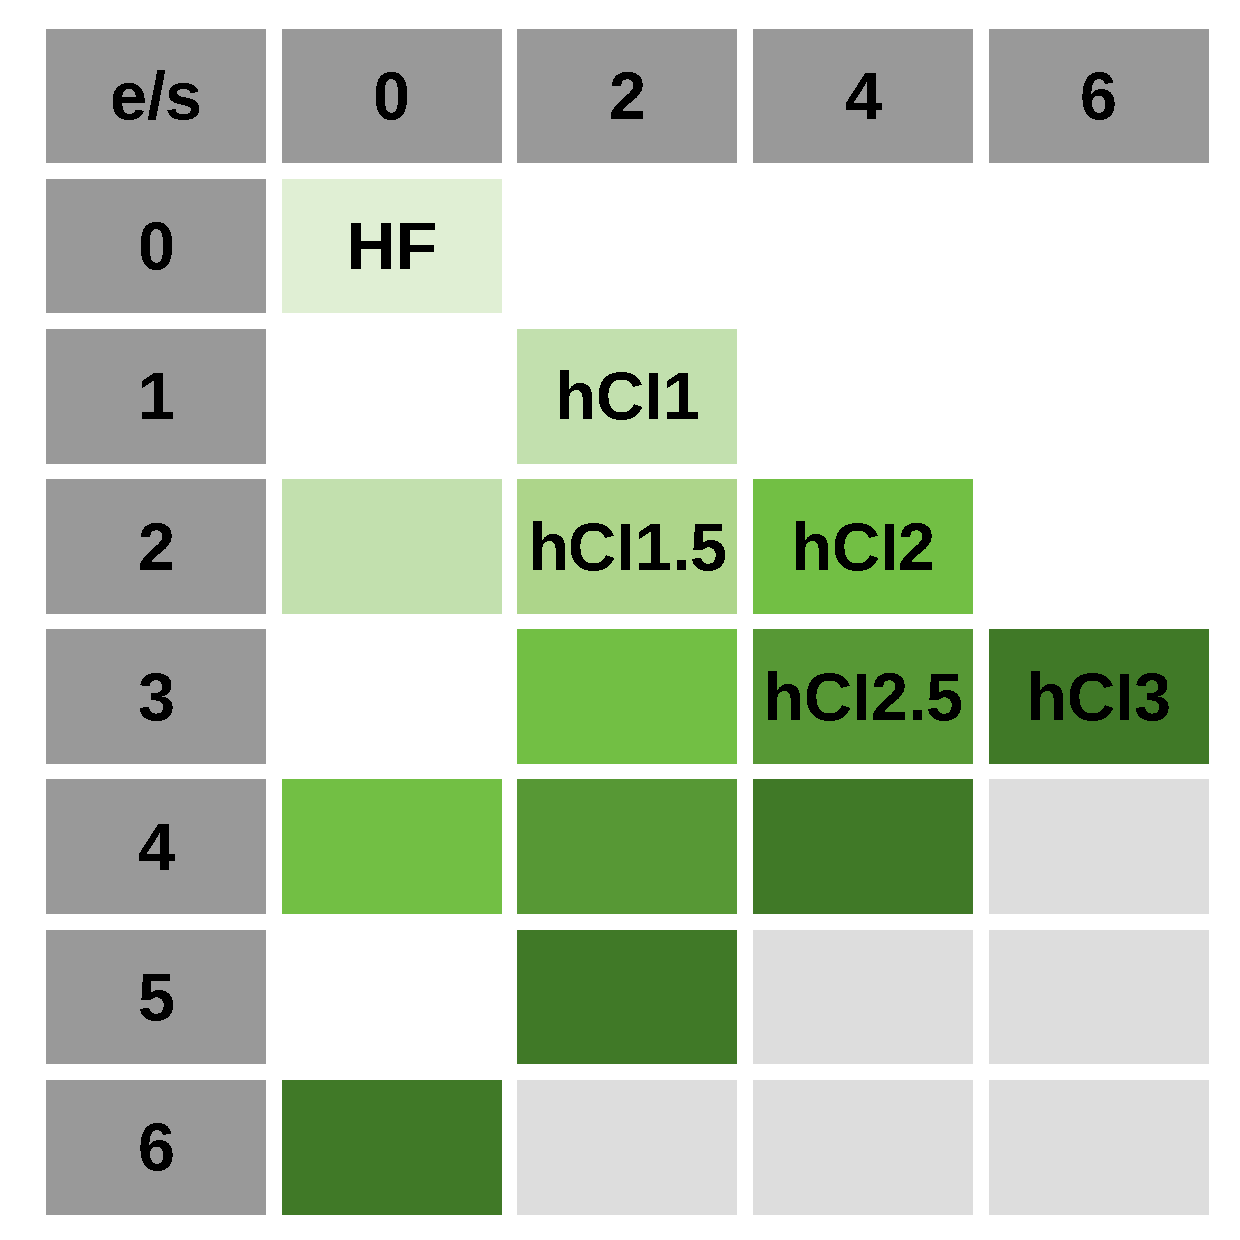
\includegraphics[width=1.0\textwidth]{fig/table_hCI},
        }
        \end{column}

        \begin{column}{0.40\textwidth}
        \begin{block}{Dissociation of \ce{F2}/cc-pVDZ}
        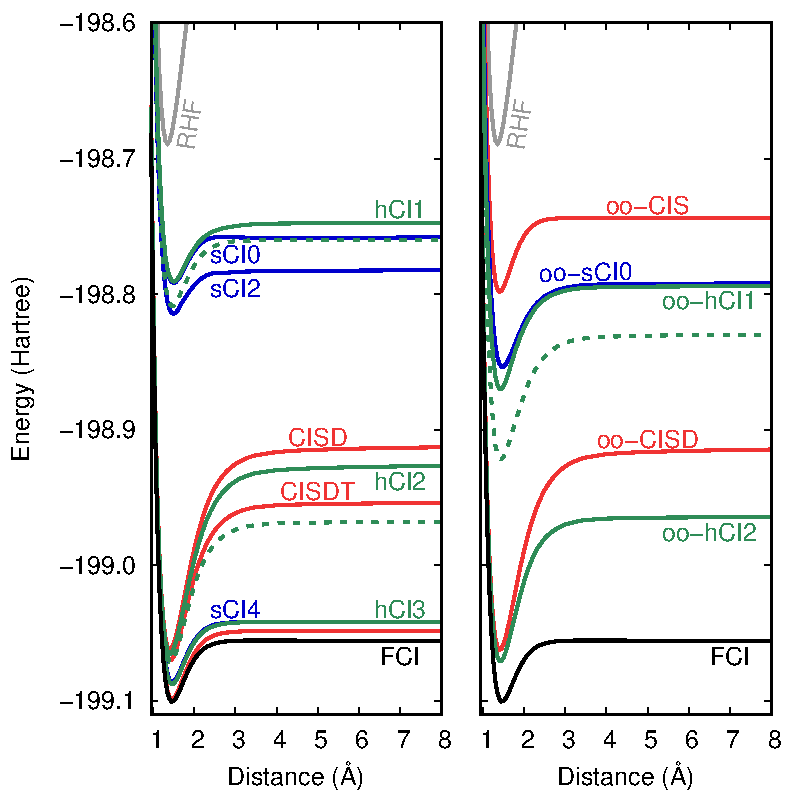
\includegraphics[width=1.00\textwidth]{fig/F2_pes.pdf}
        \end{block}
        \end{column}

        \end{columns}

\end{frame}
%%%%%%%%%%%%%%%%%%%%%%%%%%%%%%%%%%%%%%%%%%%%

%%%%%%%%%%%%%%%%%%%%%%%%%%%%%%%%%%%%%%%%%%%%
\begin{frame}{Excited states, electrons, and photons}

        \begin{columns}
        \begin{column}{0.33\textwidth}
        \centering
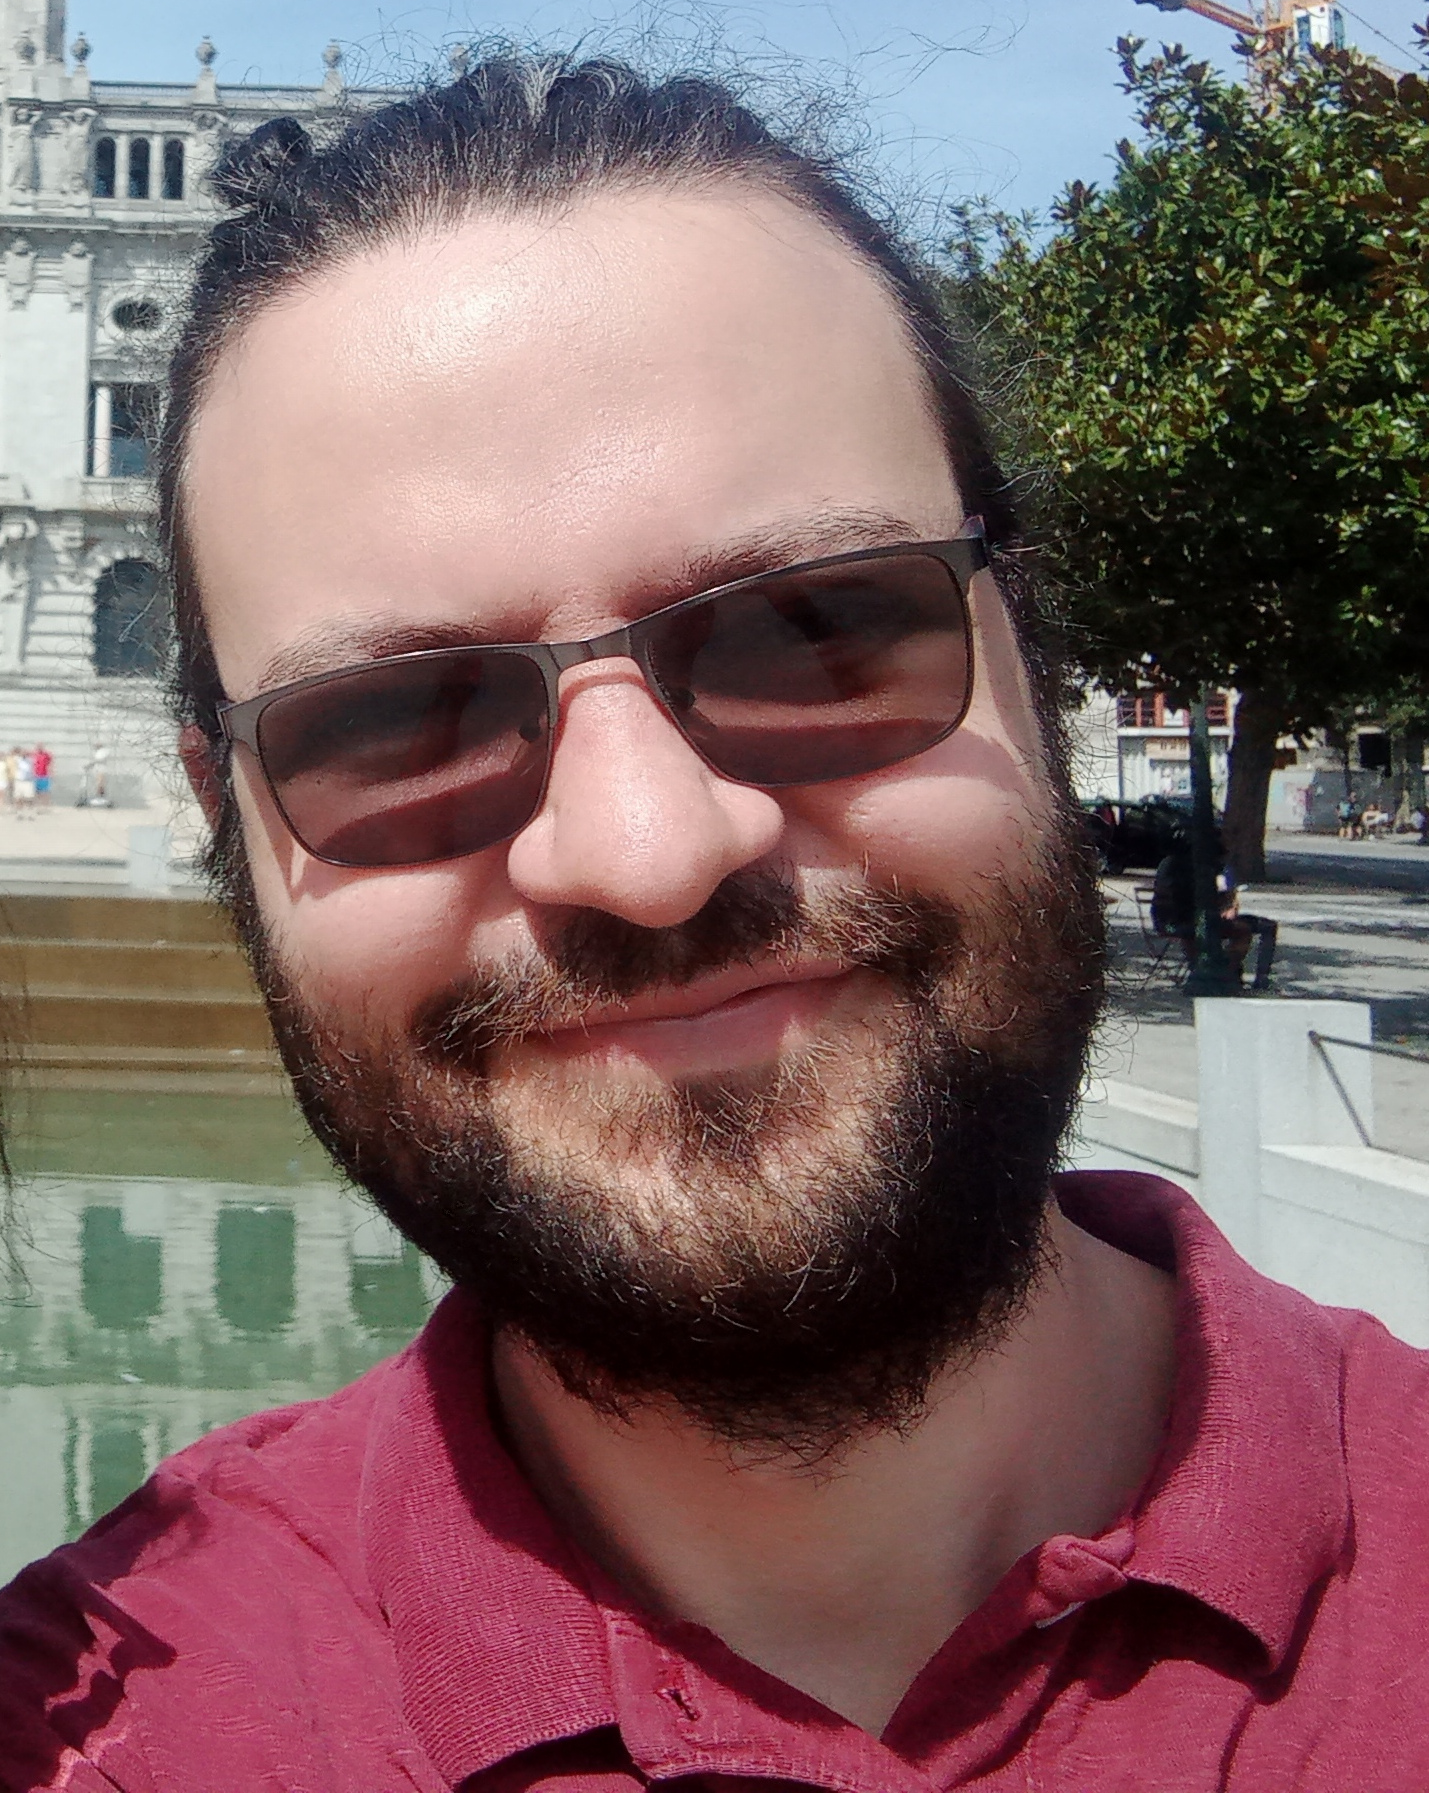
\includegraphics[width=0.46\textwidth]{fig/Fabris_2021.png}
\\
Fábris Kossoski
\\
\bigskip
        \begin{block}{Electronic structure methods}
		\bigskip
		\begin{itemize}
		\item
		{\bf State-specific methods}
		\\
		\bigskip
		\item
		{\bf Number of excited electrons}
		\end{itemize}
        \end{block}
        \end{column}

        \begin{column}{0.32\textwidth}
		\vspace{-0.5cm}
	\begin{block}{Electron-molecule scattering}
 		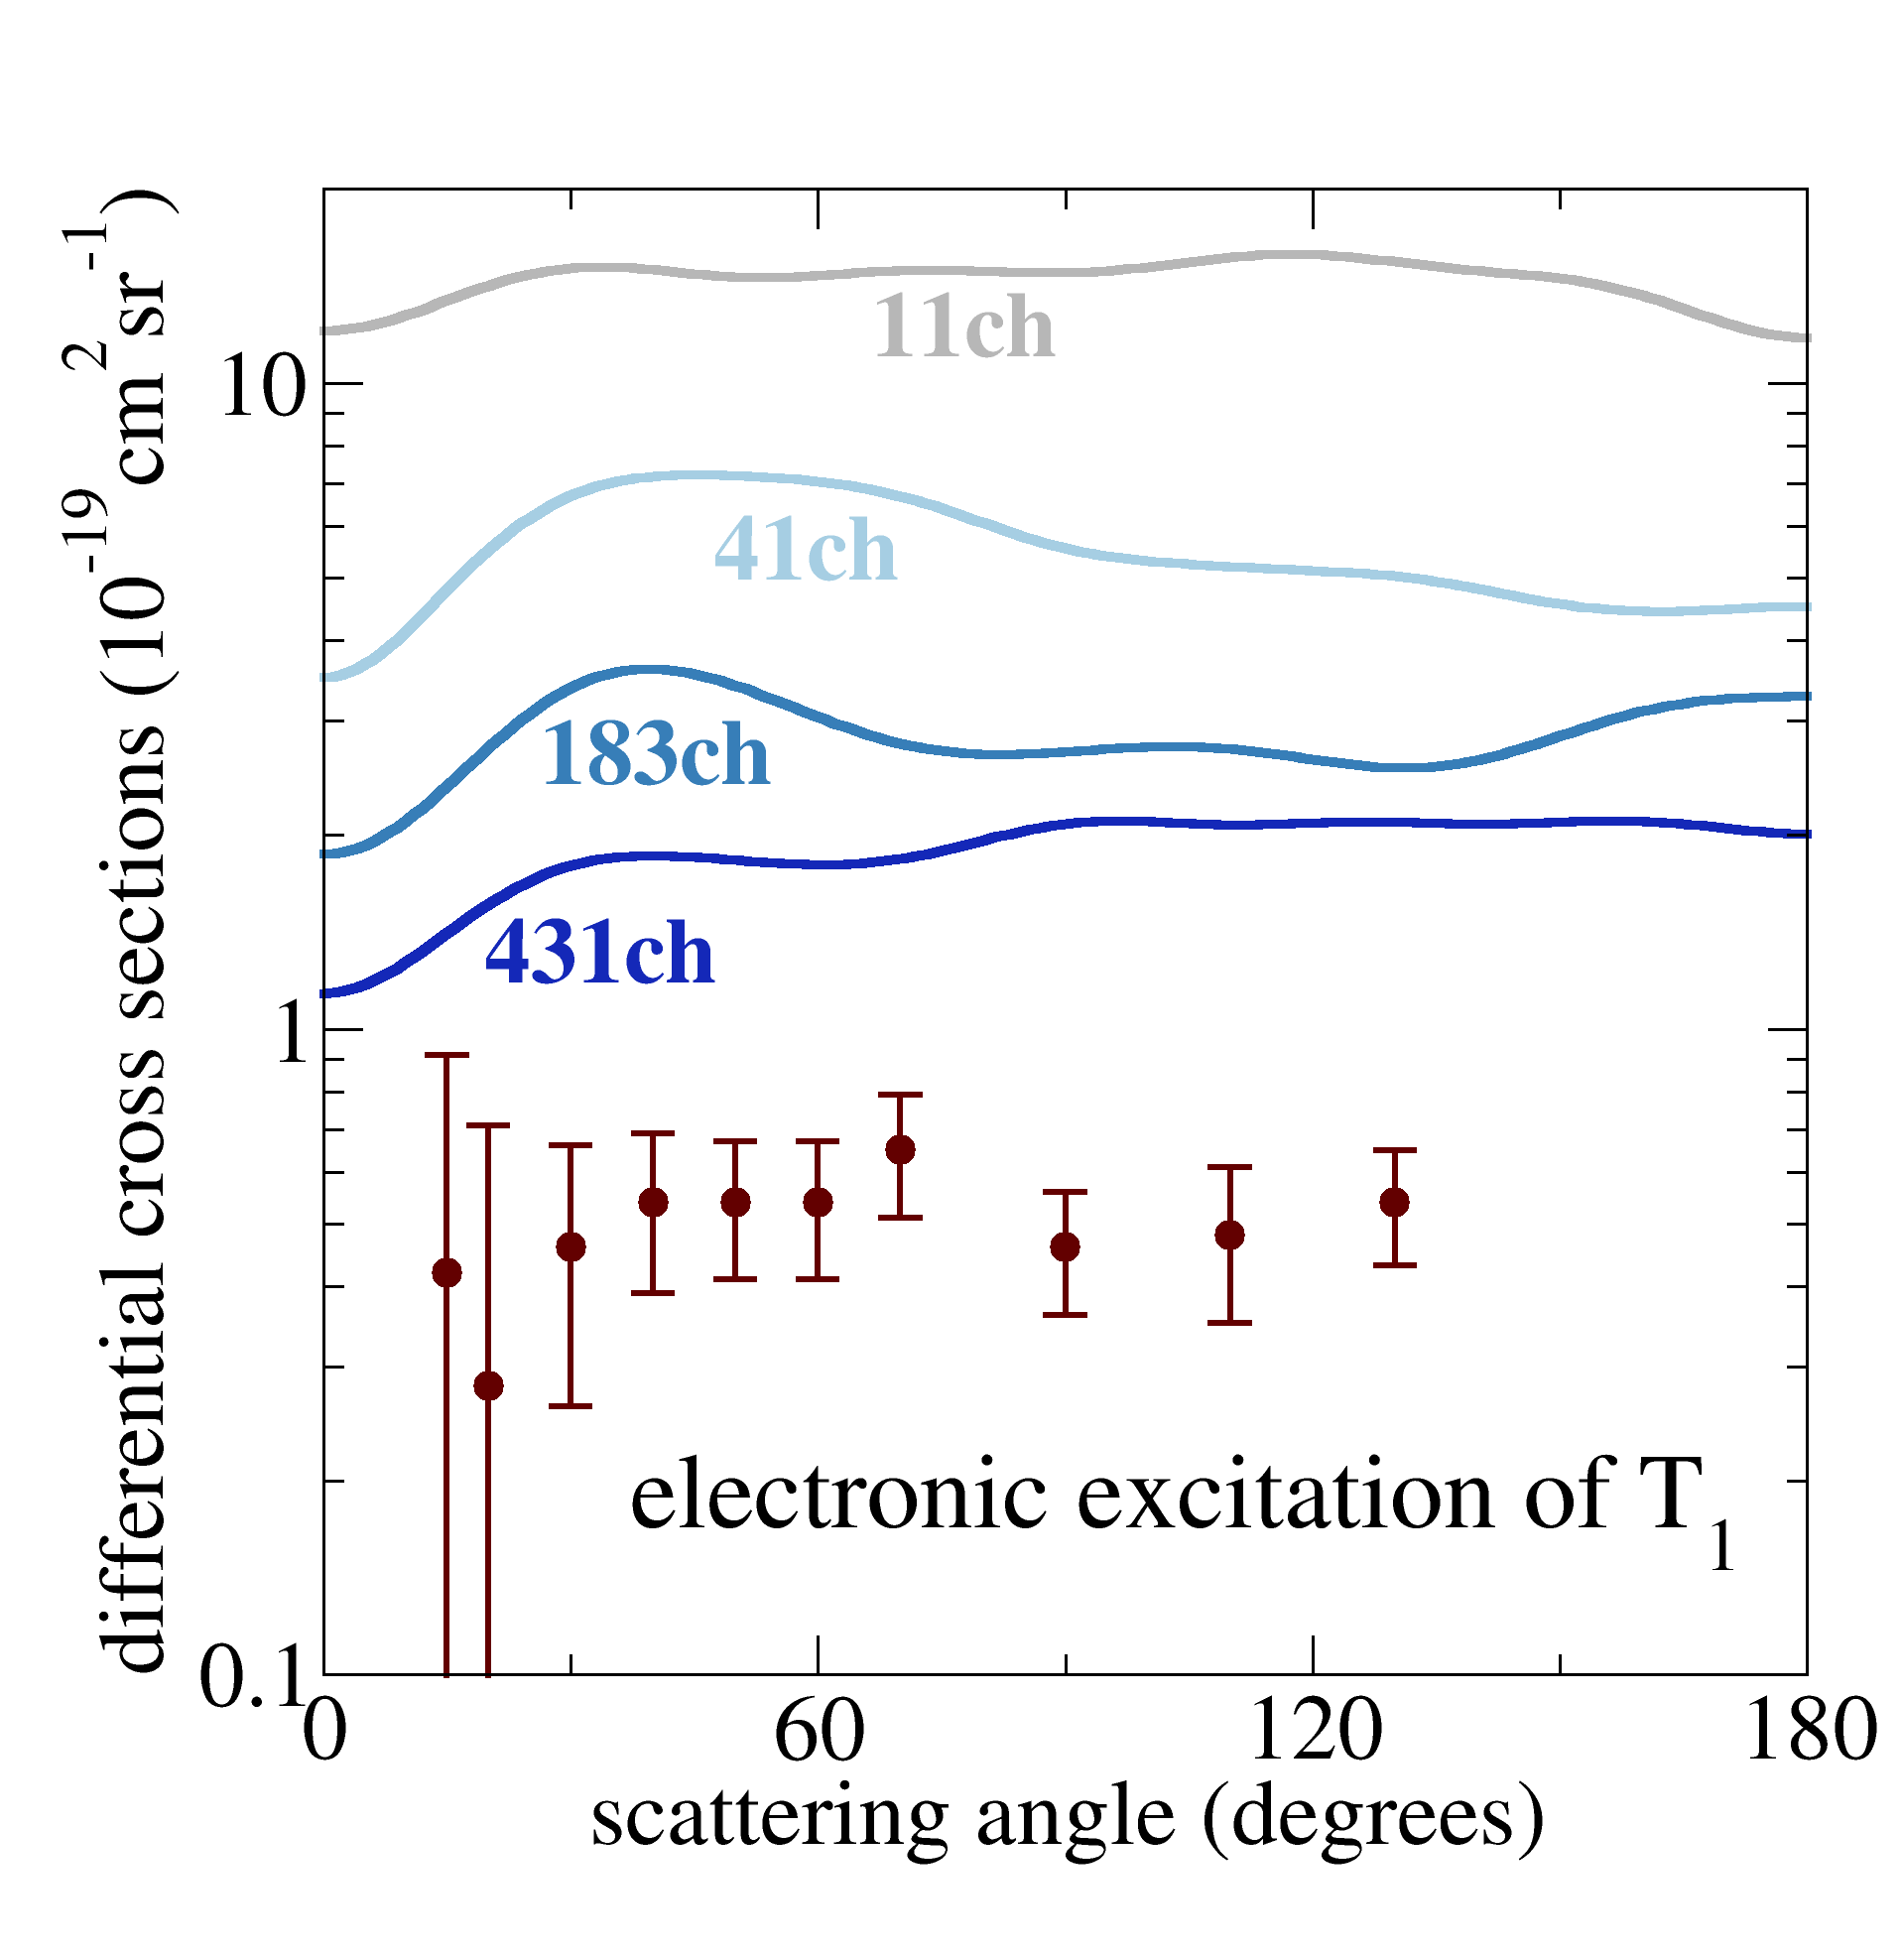
\includegraphics[width=0.90\textwidth]{fig/ethanol.png}
		\pub{PCCP 23, 17616 (2021)}
%		\\
%		\pub{EPJD 75, 310 (2021)}
		\\
		\pub{JCP 152, 244302 (2020)}
		\\
        \end{block}

        \end{column}

        \begin{column}{0.32\textwidth}
		\vspace{-0.5cm}
	\begin{block}{Nonadiabatic dynamics of resonances}
 	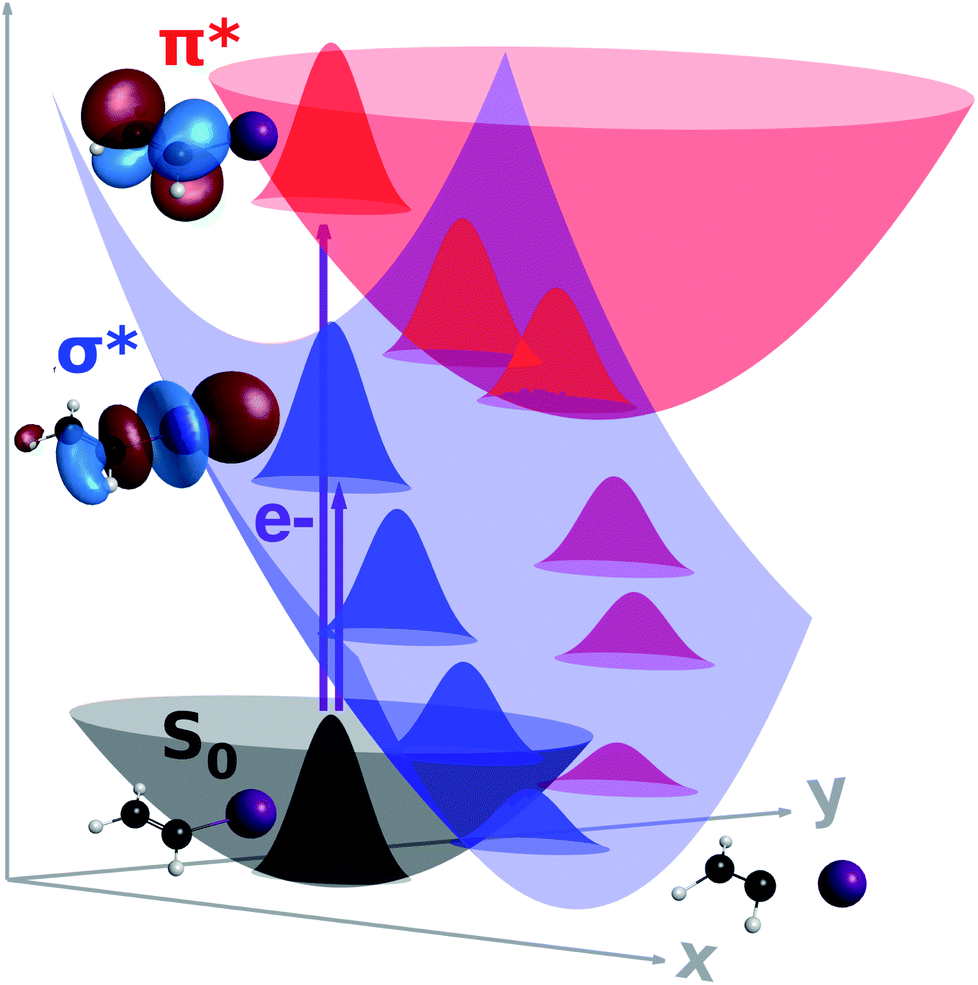
\includegraphics[width=0.9\textwidth]{fig/pes_complex.png}
	\pub{Chem. Sci., 11, 9827 (2020)}
		\\
	\pub{JCP 151, 224104 (2019)}
        \end{block}

        \end{column}

        \end{columns}

        \begin{columns}
        \begin{column}{0.32\textwidth}
        \end{column}

        \begin{column}{0.68\textwidth}
		\vspace{-0.5cm}
 	\begin{block}{VUV photoabsorption}
		\pub{PCCP 23, 2141 (2021)}
		\hspace{2cm}
		\pub{IJMS 22, 6460 (2021)}
        \end{block}
        \end{column}
        \end{columns}

\end{frame}
%%%%%%%%%%%%%%%%%%%%%%%%%%%%%%%%%%%%%%%%%%%%


%%%%%%%%%%%%%%%%%%%%%%%%%%%%%%%%%%%%%%%%%%%%
\begin{frame}{Acknowledgements}
        \begin{columns}
                \begin{column}{0.6\textwidth}
                        \begin{itemize}
				\item Pierre-François Loos (Titou)
				\vspace{0.1cm}
				\item Anthony Scemama
				\vspace{0.1cm}
				\item Michel Caffarel
				\vspace{0.1cm}
                                \item Raul Quintero 
				\vspace{0.1cm}
                                \item Clotilde Marut 
				\vspace{0.1cm}
                                \item Enzo Monino 
				\vspace{0.1cm}
                                \item Roberto Orlando 
				\vspace{0.1cm}
                                \item Yann Damour 
				\vspace{0.1cm}
                                \item Antoine Marie 
                        \end{itemize}
                \end{column}
                \begin{column}{0.32\textwidth}
                        \begin{center}
                                
\includegraphics[width=0.6\textwidth]{fig/LCPQ}
                                \\
                                
\includegraphics[width=0.5\textwidth]{fig/UPS}
                                
\includegraphics[width=0.2\textwidth]{fig/CNRS}
                                \\
                                
\includegraphics[width=0.8\textwidth]{fig/NEXT}
                                \\
                                
\includegraphics[width=\textwidth]{fig/ERC}
                        \end{center}
                \end{column}
        \end{columns}
\end{frame}
%%%%%%%%%%%%%%%%%%%%%%%%%%%%%%%%%%%%%%%%%%%%


%%%%%%%%%%%%%%%%%%%%%%%%%%%%%%%%%%%%%%%%%%%%
\begin{frame}{General overview of the PTEROSOR team}
        \centering
        \begin{columns}
                \begin{column}{0.325\textwidth}
                        \centering
                        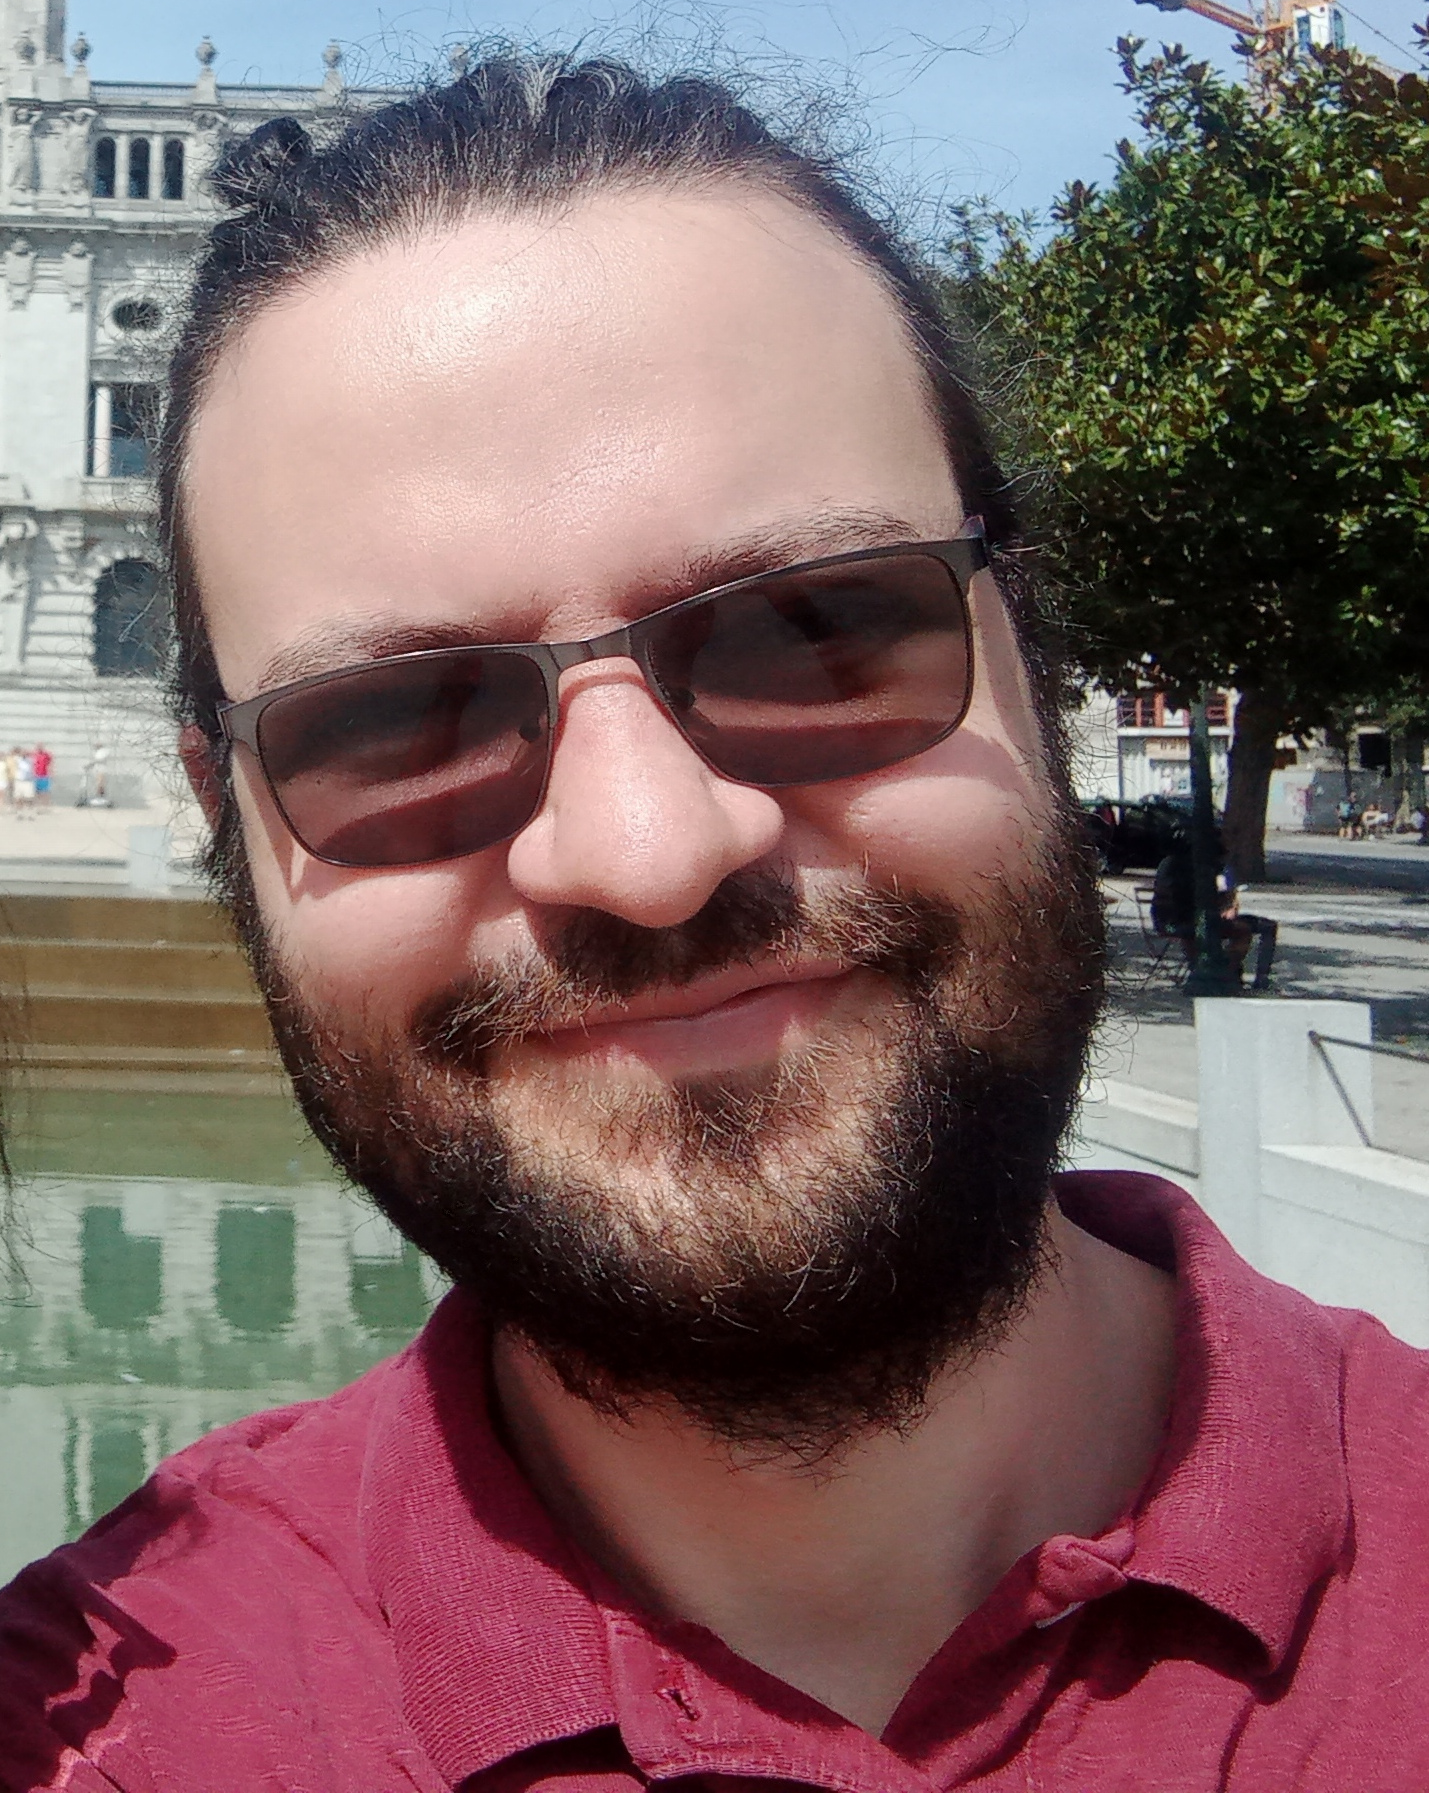
\includegraphics[width=0.3\textwidth]{fig/Fabris_2021.png}
                        \\
                        F\'abris Kossoski
                        \\
                        \vspace{0.25cm}
                        \includegraphics[width=0.3\textwidth]{fig/Yann.jpg}
                        \\
                        Yann Damour
                        \\
                        \vspace{0.25cm}
                        \includegraphics[width=0.3\textwidth]{fig/Enzo}
                        \\
                        Enzo Monino
                        \\
                \end{column}
                \begin{column}{0.50\textwidth}
                         \vspace{-0.5cm}
                \smartdiagramset{distance planet-satellite=4cm}
                        \resizebox{\textwidth}{!}{
                                \smartdiagram[constellation diagram]{
                                        {\small Excited-State Methods (Anthony, Michel \& Titou)},
                                        {\small Selected CI (Yann \& Fabris) },
                                        {\small CC for Excited States (Antoine, Raul \& Fabris)},
                                        {\small ``Complex'' Quantum Chemistry (Antoine)},
                                        {\small Many-Body Perturbation Theory (Enzo \& Roberto)},
                                        {\small Ensemble DFT (Clotilde)},
                                        {\small QUEST database (Mika, Martial \& co)}
                                }
                        }
                \end{column}
                \begin{column}{0.325\textwidth}
                        \centering
                        \includegraphics[width=0.2\textwidth]{fig/Raul}
                        \\
                        Raul Quintero
                        \\
                        \vspace{0.25cm}
                        \includegraphics[width=0.3\textwidth]{fig/Roberto}
                        \\
                        Roberto Orlando
                        \\
                        \vspace{0.25cm}
                        \includegraphics[width=0.3\textwidth]{fig/Clotilde}
                        \\
                        Clotilde Marut
                        \\
                \end{column}
        \end{columns}
                        \vspace{-0.5cm}
        \url{https://lcpq.github.io/PTEROSOR/}
\end{frame}
%%%%%%%%%%%%%%%%%%%%%%%%%%%%%%%%%%%%%%%%%%%%


\end{document}
